\documentclass[11pt,          % font size: 11pt or 12pt
               phd,           % degree:    ms or phd
               onehalfspacing % spacing: onehalfspacing or doublespacing
               ]{ncsuthesis}

%%----------------------------------------------------------------------------%%
%%------------------------------ Import Packages -----------------------------%%
%%----------------------------------------------------------------------------%%

\usepackage{booktabs}  % professionally typeset tables
\usepackage{amsmath}
\usepackage{textcomp}  % better copyright sign, among other things
\usepackage{xcolor}
\usepackage{lipsum}    % filler text
\usepackage{subfig}    % composite figures
\usepackage{multirow}
\usepackage{url}


%%----------------------------------------------------------------------------%%
%%---------------------------- Formatting Options ----------------------------%%
%%----------------------------------------------------------------------------%%
%%

%% -------------------------------------------------------------------------- %%
%% Disposition format -- any titles, headings, section titles
%%  These formatting commands affect all headings, titles, headings,
%%  so sizing commands should not be used here.
%%  Formatting options to consider are
%%     +  \sffamily - sans serif fonts.  Dispositions are often typeset in
%%                    sans serif, so this is a good option. 
%%     +  \rmfamily - serif fonts
%%     +  \bfseries - bold face
%\dispositionformat{\sffamily\bfseries}   % bold and sans serif
\dispositionformat{\bfseries}            % bold and serif

%% -------------------------------------------------------------------------- %%
%% Formatting for centered headings - Abstract, Dedication, etc. headings
%%  This is where one might put a sizing command.
%%  \MakeUppercase can be used to typeset all headings in uppercase.
\headingformat{\large\MakeUppercase}   % All letters uppercase
%\headingformat{\large}                % Not all uppercase
%\headingformat{\Large\scshape}        % Small Caps, used with serif fonts.

%% Typographers recommend using a normal inter-word space after
%% sentences. TeX's default is to add an wider space, but \frenchspacing
%% gives a normal spacing. Comment out the following line if you prefer
%% wider spaces between sentences.
\frenchspacing


%% -------------------------------------------------------------------------- %%
%%  Optional packages
%%    A number of compatible packages to improve the look and feel of
%%    your document are available in the file optional.tex 
%%    (For example, hyperlinks, fancy chapter headings, and fonts)
%% To use these options, uncomment the next line and see optional.tex
%%%  Optional Packages to consider.   These packages are compatible with
%%    ncsuthesis.  

%% -------------------------------------------------------------------------- %%
%% Fancy chapter headings
%%  available options: Sonny, Lenny, Glenn, Conny, Rejne, Bjarne
\usepackage[Sonny]{fncychap}

%%----------------------------------------------------------------------------%%
%% Hyperref package creates PDF metadata and hyperlinks in Table of Contents
%%  and citations.  Based on feedback from the NCSU thesis editor, 
%%  the links are not visually distinct from normal text (i.e. no change
%%  in color or extra boxes).
\usepackage[
  pdfauthor={John Mark Smith},
  pdftitle={The Title},
  pdfcreator={pdftex},
  pdfsubject={NC State ETD Thesis},
  pdfkeywords={keyword1, keyword2},
  colorlinks=true,
  linkcolor=black,
  citecolor=black,
  filecolor=black,
  urlcolor=black,
]{hyperref}


%% -------------------------------------------------------------------------- %%
%% Microtype - If you use pdfTeX to compile your thesis, you can use
%%              the microtype package to access advanced typographic
%%              features.  By default, using the microtype package enables
%%              character protrusion (placing glyphs a hair past the right 
%%              margin to make a visually straighter edge)
%%              and font expansion (adjusting font width slightly to get 
%%              more favorable justification).
%%              Using microtype should decrease the number of lines
%%              ending in hyphens.
\usepackage{microtype}


%%----------------------------------------------------------------------------%%
%% Fonts 

%% ETD guidelines don't specify the font.  You can enable the fonts
%%  by uncommenting the appropriate lines.  Using the default Computer 
%%  Modern fonts is *not* required.  A few common choices are below.
%%  See http://www.tug.dk/FontCatalogue/ for more options.

%% Serif Fonts -------------------------------------------------
%%  The four serif fonts listed here (Utopia, Palatino, Kerkis,
%%  and Times) all have math support.


%% Utopia
\usepackage[T1]{fontenc}
\usepackage[adobe-utopia]{mathdesign}

%% Palatino
%\usepackage[T1]{fontenc}
%\usepackage[sc]{mathpazo}
%\linespread{1.05}

%% Kerkis
%\usepackage[T1]{fontenc}
%\usepackage{kmath,kerkis}

%% Times
%\usepackage[T1]{fontenc}
%\usepackage{mathptmx}


%% Sans serif fonts -------------------------

%\usepackage[scaled]{helvet}  % Helvetica
%\usepackage[scaled]{berasans} % Bera Sans



%%----------------------------------------------------------------------------%%
%%---------------------------- Content Options -------------------------------%%
%%----------------------------------------------------------------------------%%
%% Size of committee: 3, 4, 5, or 6 -- this number includes the chair
\committeesize{3}

%% Members of committee
%%  Each of the following member commands takes an optional argument
%%   to specify their role on the committee.
%%  For co-chairs, use the commands:
%%      \cochairI{Doug Dodd}
%%      \cochairII{Chris Cox}
%%
\chair{Vincent Freeh}
\memberI{Xipeng Shen}
\memberII{William Enck}


%% Student writing thesis, \student{First Middle}{Last}
\student{Zhuowei}{Wang} % a full middle name
%\student{John M.}{Smith} % a middle initial

%% Degree program
\program{Computer Science}

%% Thesis Title
%%  Keep in mind, according to ETD guidelines:
%%    +  Capitalize first letter of important words.
%%    +  Use inverted pyramid shape if title spans more than one line.
%%
%%  Note: To break the title onto multiple lines, use \break instead of \\.
\thesistitle{Design and Implementation \break
of \break
a Distributed Snapshot File System}

%% Degree year.  Necessary if your degree year doesn't equal the current year.
\degreeyear{2014}


%%----------------------------------------------------------------------------%%
%%---------------------------- Personal Macros -------------------------------%%
%%----------------------------------------------------------------------------%%

%% A central location to add your favorite macros.

%% A few examples to get you started.
\newcommand{\uv}[1]{\ensuremath{\mathbf{\hat{#1}}}}
\newcommand{\bo}{\ensuremath{\boldsymbol{\Omega}}}
\newcommand{\eref}[1]{Eq.~\ref{#1}}
\newcommand{\fref}[1]{Figure~\ref{#1}}
\newcommand{\tref}[1]{Table~\ref{#1}}
\newcommand{\cref}[1]{Chapter~\ref{#1}}

%%---------------------------------------------------------------------------%%
\begin{document}

%%---------------------------------------------------------------------------%%
\frontmatter

%% ------------------------------ Abstract ---------------------------------- %%
\begin{abstract}

%\lipsum[1-6]


\end{abstract}


%% ---------------------------- Copyright page ------------------------------ %%
%% Comment the next line if you don't want the copyright page included.
\makecopyrightpage

%% -------------------------------- Title page ------------------------------ %%
\maketitlepage

%% -------------------------------- Dedication ------------------------------ %%
\begin{dedication}
 \centering To my parents.
\end{dedication}

%% -------------------------------- Biography ------------------------------- %%
\begin{biography}
The author was born in a small town \ldots
\end{biography}

%% ----------------------------- Acknowledgements --------------------------- %%
\begin{acknowledgements}
I would like to thank my advisor for his help.
\end{acknowledgements}


\thesistableofcontents

\thesislistoftables

\thesislistoffigures


%%---------------------------------------------------------------------------%%
\mainmatter

\chapter{Introduction}
\label{chap:intro}

    Mention ``file system'' and what usually comes to mind are disk file systems like FAT32~\cite{fat_wiki} or Ext4~\cite{ext4}, for disks are the most common persistent storage. In addition, file systems can be used to access data from remote machine for example NFS~\cite{nfs}, can be used to access non-traditional form of data and storage spaces for instance GmailFS~\cite{gmailfs, gmailfs2}, can also provide useful and transparent functionalities like encryption, compression or soft-RAID~\cite{encrypt, compression}.

    As the network bandwidth increases, we no longer have to keep our data on local disk. Nowadays more and more data are stored online. Individuals are uploading their personal data to web services; commercial companies are using cloud storage systems like Amazon S3 to store their data remotely. There are a large number of reasons to store data in the cloud. It makes sharing and collaboration easier and ensures that the data can be accessed by its owner anywhere and anytime. Though there are lots of services and applications that help us to access data online, a network file system is able to make this process totally transparent to the user and user programs. A distributed file system can also maps different machines into a logically unified volume while providing features like redundancy and load balancing. Popular distributed file systems adopted by industry and academic institutes include NFS and AFS~\cite{afs}.

    NoSQL databases~\cite{nosql} are used for store and retrieve data which is modeled differently from the tabular relations. They provide alternatives to classic relational databases, bring innovation and new ideas to the community, industry and academia. Commercial companies like Google and Amazon have been using them in production environments for many years. Compared to relational databases, they have many advantages in performance, scalability and flexibility whereas low functionality, e.g. not normalized data and poor transaction support~\cite{transaction}, is their disadvantage.

    We believe a document oriented NoSQL database~\cite{docdb} can serve as a backend of the file system to store and manage the actual data. Because a file system needs to ensure consistency and query single entity (file, directory) but not much demand of join queries and join updates. A document oriented NoSQL database that focuses on performance, scalability and flexibility rather than the relational algebra may be a better fit to this task. In addition, the high scalability of NoSQL database makes it easy to distribute the storage on to different machine~\cite{sharding}.

    Furthermore, when the file system is released from the burden of on disk resource management by using a database as backend, developers can put more efforts toward other features of the file system such as snapshot and deduplication. A snapshot subsystem is useful. It can be used to test installations, keep track of modifications, provide a rollback mechanism, and make the backup process more efficient. It is becoming more and more popular for a modern file system to have the capability to take snapshots. For instance, from FAT to NTFS~\cite{ntfs} and from Ext2~\cite{ext2_wiki} to Ext4, more and more file systems have this feature built-in. Ground breaking file system ZFS~\cite{zfs_wiki} and experimental file system BTRFS~\cite{btrfs} all come with snapshot capability. Deduplication is another popular feature, where the file system try to identify duplicated data and eliminate them in order to save storage space.

\section{Contribution}

    We design a new distributed snapshot file system and study the way to improve its performance. We use MongoDB as a backend of the file system to improve the network performance and reliability. We introduce rsync algorithm into the file system and use it to improve the network performance and snapshot efficiency, by identifying the duplicated data between remote and local and between snapshots. In addition, we use a new design of snapshot system which is called patch-based snapshot. 

    We vaildate our design by implemenating it and testing it. The test results indicate that the file system we proposed has a comparable performance to the popular network file system NFS. Furthermore, it shows that the rsync enhanced copy-on-write snapshot system can boost the space efficiency of the snapshot system compared to classic copy-on-write snapshot system.

    In this thesis, we propose a new design of distributed file system with snapshot capability. We have the design implemented by Java, MongoDB, FUSE, and other techniques. We also propose several new ways to improve the efficiency of the file system. We tested and compared the performance of our implantation with other file systems, studied the snapshot system performance under different scenarios, compare and explain the outcome of tests.

\chapter{Related work}
\label{chap:related_work}

    There are important prior work in customized file systems, NoSQL database, and snapshots. Several of them are related to this thesis and they are summarized in this chapter.

\section{POSIX}

    POSIX (Portable Operating System Interface), is a family of IEEE standard for operating systems~\cite{posix_wiki}. It influences the design of many modern operating system (e.g., Linux, Windows NT, Mac). The POSIX standard defines a standard environment for operating system (process, user, file, directory, etc.) along with a set of APIs for user program (like fork, exec, I/O functions, etc.)~\cite{posix}. Some file format standard (e.g., tar) and some shell utilities (e.g. awk, vi) are also included in the standard. The purpose of this standard is to maintain compatibility between operating system such that a user program written for one POSIX operating system will work on any POSIX operating system theoretically. 

    The POSIX standard specifies a set of file system APIs that defines file and directory operations. Any file system that implements this set of APIs should be compatible with operating systems that follows POSIX standard.

\section{FUSE}

    FUSE, the Filesystem in User Space, is a developer framework for file system. It was originally developed for AVFS (virtual file system that allows all users
to look inside archived or compressed files, or access remote files)~\cite{avfs} but has become a separate project. It has now been adopted into the Linux kernel and has many ports on other Unix-like operating systems. FUSE provides a programming interface that is very similar to POSIX file operations. A file system with this interface can get file system calls from kernel module VFS (the Virtual File System)~\cite{vfs}. Such that a user programs is able to use standard file system call to access it as if the file system is supported by operating system natively. By running the file system in user space, FUSE isolates the file system from operating system. In such a way, developers of the file system do not need to understand complicated kernel code or to debug in the kernel~\cite{fuse}.

    FUSE routes the file system call from VFS in kernel space back to the user space and then lets the user program to process the file system call. It is a widely used component of Linux file system. A number of well-known projects are using FUSE, for example the OverlayFS, ntfs-3g, and vmware tools. Inspired by FUSE, there are some other user space file system like Dokan under windows.

    There are different language bindings of FUSE. Our implementation is built on the Java bindings FUSE-JNA. The FUSE-JNA is a recent active project developed by Etienne Perot. The author describes his project as ``No-nonsense, actually-working Java bindings to FUSE using JNA''~\cite{fusejna}. Other Java bindings of FUSE include FUSE-J, jnetfs~\cite{jnetfs}.

\section{MongoDB}

    MongoDB is a document oriented NoSQL distributed database~\cite{mongo_overview}. It focuses on scalability, performance and availability~\cite{mongo_overview}. Document oriented storage that can store semi-structured data makes it flexible and makes it suitable for agile development~\cite{docdb}. In addition, MongoDB also provides features like load balancing and replication. These features make MongoDB an ideal backend for a distributed file system. Developers have already built a file storage system called GridFS using MongoDB which provides a mechanism to store and retrieve file of any size~\cite{gridfs}.

    MongoDB represents document in JSON (JavaScript Object Notation) format. JSON is a open, human and machine-readable standard that facilitates data interchange. Behind the scenes, MongoDB uses BSON (Binary JSON) to encode and store the documents. Both JSON and BSON format supports embedding object and arrays within other objects and arrays. MongoDB can query and build index not only on top level keys but also nested objects. The developer believes this will grant users of MongoDB ease of use and flexibility together with the speed and richness of a lightweight binary format~\cite{bson}.

    MongoDB is one of the most popular NoSQL database. It has a large and active developer community. A recent \$150 million investment ensures the long term support and reflects the confidence of investors~\cite{mongInvest}.

\section{Snapshot}

    A snapshot is a state of a system at a particular point in timer~\cite{btrfscow}. They can be either read-only or writable. Writable snapshots are also called clones. They are supported by several advanced file system like ZFS and BTRFS. The Ext4 file system also has a development branch for writable snapshot. From the user’s point of view, a read-only snapshot is an immutable and exact copy of the file system at a specific time, whereas a writable snapshot is a fork of the file system at a particular time spot. A writable snapshot allows modification to snapshots but modifications to a snapshot are separate from the origin and other snapshots. (i.e., changes to the snapshot cannot be seen in other snapshots or the origin and vice versa) With the help of writable snapshot, one can easily create and switch between different file system branch and make changes to them without affecting other branch. Writable snapshots can also provide file system isolation for process, software or virtual machine.

\section{Copy-on-Write}

    Copy-on-write is a strategy widely used in computer science. A program that uses copy-on-write strategy accesses data though a pointer or a reference. When a copy operation is requested, instead of making a copy of actual data, a program that uses copy-on-write strategy will simply return a new reference to the original data. Only when a modification to one of the ``copies'' is requested, the program will then make an actual copy of the original data and then apply the modification to that copy. At the end, the program will point corresponding pointer or reference to the updated copy. This design not only eliminates unnecessary overhead in data copy but also ensures consistency, integrity and an easy support of transactions. In addition to those benefits, a file system using copy-on-write strategy will be able to take snapshots with low overhead. Without copy-on-write strategy, snapshots either write in-place which is more expensive, or requires special architecture in storage system like the Split-Mirror architecture.

\section{Existing Snapshot Storage Systems}

    Snapshot is an important features of a storage system. Existing works include LVM snapshot, SnapFS, OverlayFS, ZFS, BTRFS, and Ext4.
    
    The LVM snapshot is a snapshot system included in the logical volume manager~\cite{lvm, disk_perform_lvm}. It takes snapshot of blocks in the logical volume and gives snapshots capability to any file system build upon the LVM system. However, as an underlying service, LVM snapshot is not aware of file structures, making it hard to find duplicate data stream and thus is less efficient in terms of disk space.
    
    SnapFS is a file system focusing on snapshots in Linux kernel~\cite{snapfs}. It is strongly coupled with its underlying Ext file system. Therefore, SnapFS is able to apply copy-on-write strategy on block but restrict its underlying file system to Ext file system family. 
    
    OverlayFS~\cite{overlayfs}, also called UnionFS, is a file system popular in embedded systems, hand held devices, PDAs and smartphones. Similar to SnapFS, OverlayFS is also built upon other file systems. But OverlayFS does not restrict the type of its underlying file system as SnapFS does. This gives OverlayFS a lot flexibility as it can adapt to any storage media that has a standard file system implemented. The OverlayFS applies copy-on-write on files and directory level.

    BTRFS~\cite{btrfs} is an experimental file system developed by Oracle. It is inspired by the well-known Solaris file system ZFS and shares a lot of similarity with ZFS. Both of them usese copy-on-write snapshots at block level granularity~\cite{btrfscow}.
    
    Ext4 file system was extended to include a snapshot subsystem that applies copy-on-write strategy on block level. A writable snapshot feature for Ext4 is currently under development by the same group of developer~\cite{ext4snap}. It is inspired by CTERA Network's NEXT3 file system which is a clone of ext3 file system with built-in support for snapshots.

\section{The Rsync Algorithm}
    
    The rsync algorithm is used in the rsync utility in Unix-like system to synchronize files though network. This algorithm is invented by Andrew Tridgell and he described the algorithm as ``for the efficient update of data over a high latency and low bandwidth link''~\cite{rsync_alg}. The algorithm calculate and compare a weak checksum of blocks between remote file and local file to identify duplicated blocks. In order to achieve efficiency, the checksum algorithm takes only O(1) time complexity to calculate based on prior results, such that checking duplication at any offset in local file is possible. The algorithm performs well in delta encoding and reduces the data transferred between remote machines.


\chapter{The File System}
\label{chap-three}
\begin{figure}[hbtp]
\centering
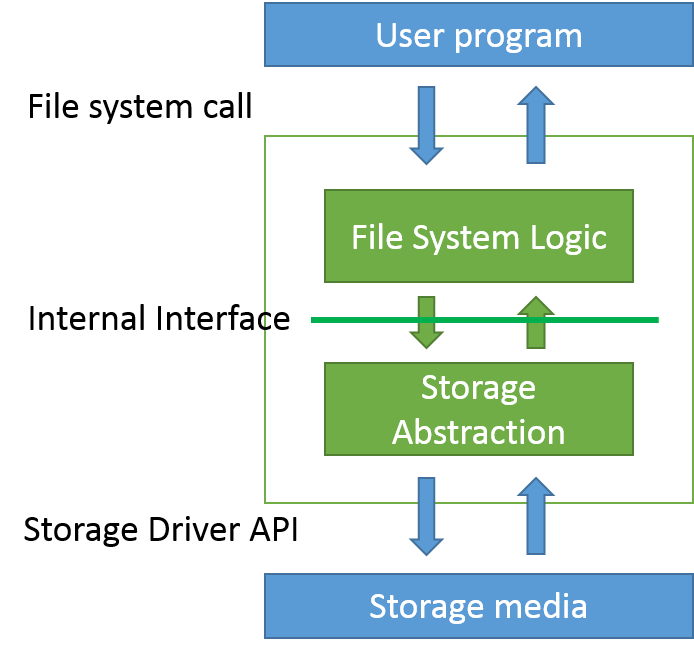
\includegraphics[width=0.5\textwidth]{Chapter-3/figs/fig8.png}
\caption{Modules of Kabi File System}
\label{fig:modules}
\end{figure}

    The file system we implemented (referred as “the Kabi File System” hereafter) can be divided into two internal modules, the storage abstraction module and the file system logic module, as shown in \fref{fig:modules}. The file system logic module decomposes any file system call to series of standard operations to the basic elements in the file system. While the storage abstraction module abstracts the underlying storage media and expose a set of method to the file system logic. There is an internal interface in between that defines several standard method to operate the basic elements. 

    The user program talks to the file system logic through file system APIs. Therefore for different file system API (e.g. FUSE, Dokan, POSIX), we will have different implementation of file system module. The storage abstraction module operates the underlying storage media through its driver, protocol or API. So an implementation of the storage media module is associate with certain storage media (e.g. MongoDB, Volume manager, Amazon S3 service). By using this design, we can easily migrate the file system to other operating system (by changing the file system logic module) or other underlying storage media (by replacing the storage abstraction module).

\begin{figure}[hbtp]
\centering
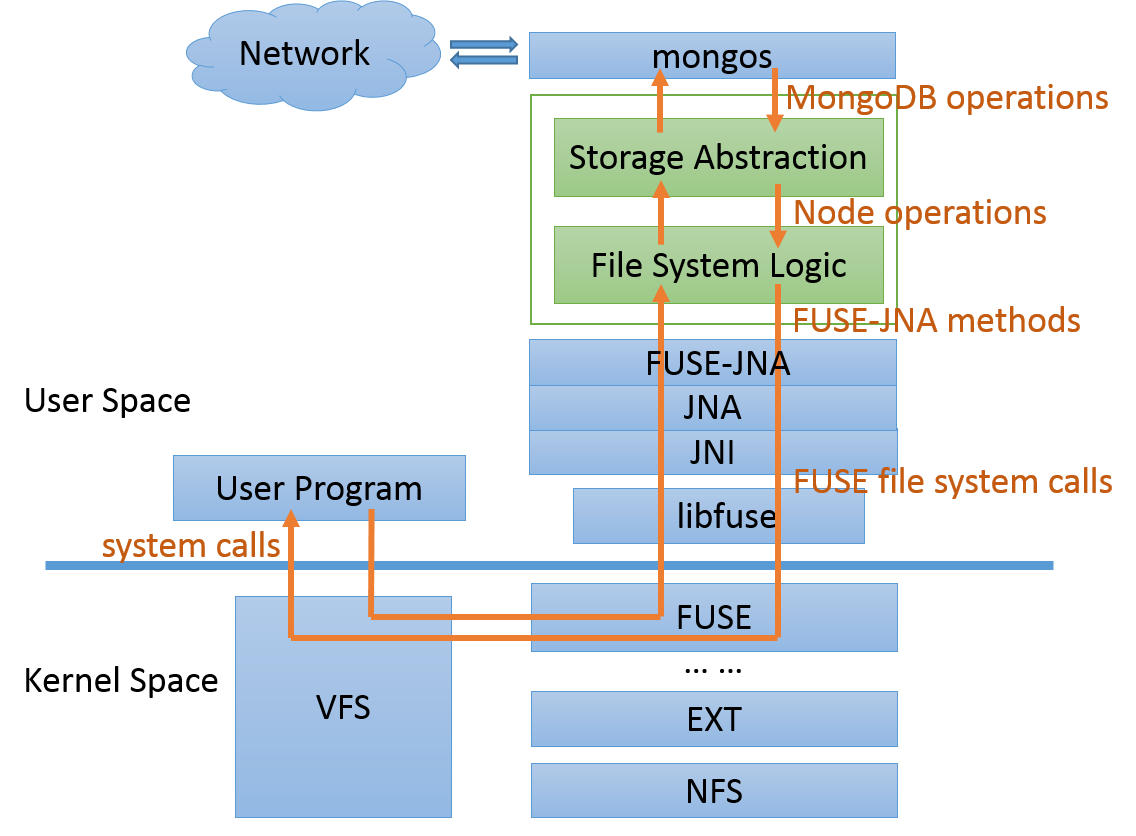
\includegraphics[width=0.8\textwidth]{Chapter-3/figs/fig1.png}
\caption{System Diagram of Kabi File System}
\label{fig:diagram}
\end{figure}

	In our proof-of-concept implementation, FUSE is used to connect the user program file system calls to the Kabi File System. A file system call from a user program will first be captured by VFS module in the kernel and routed to FUSE. FUSE will then pass on the file system call to the file system and pop the return value back to VFS module.

    In order to connect the FUSE dynamic library “libfuse”, an open source project FUSE-JNA is used to map libfuse function to Java methods. The project is slightly modified so as to keep the logging module consistent with the file system. JNA of version 3.5.2 is required by FUSE-JNA to avoid the timestamp issue.

    On the other side, the MongoDB Java driver is used by system abstraction module to communicate with the MongoDB daemon process (Mongos or Mongod).
The system diagram in \fref{fig:diagram} shows the relationship between the file system, MongoDB and operating system.

    On file system initialization, an integer parameter specifying the block size in bytes must be provided. Some optional parameter include the name of the MongoDB collection used by the file system. These parameters provided on initialization will be stored in a special MongoDB collection.

    The file system also requires a JSON format ASCII configuration file on mount. The configuration file should have three sections, specifying the FUSE options, MongoDB options and file system client options. These parameters are important to specify the data source (such as the ip address and server status of MongoDB server), the snapshot to be mounted and the name of the MongoDB collection where the initialization parameter is written.
    
\begin{figure}[hbtp]
\centering
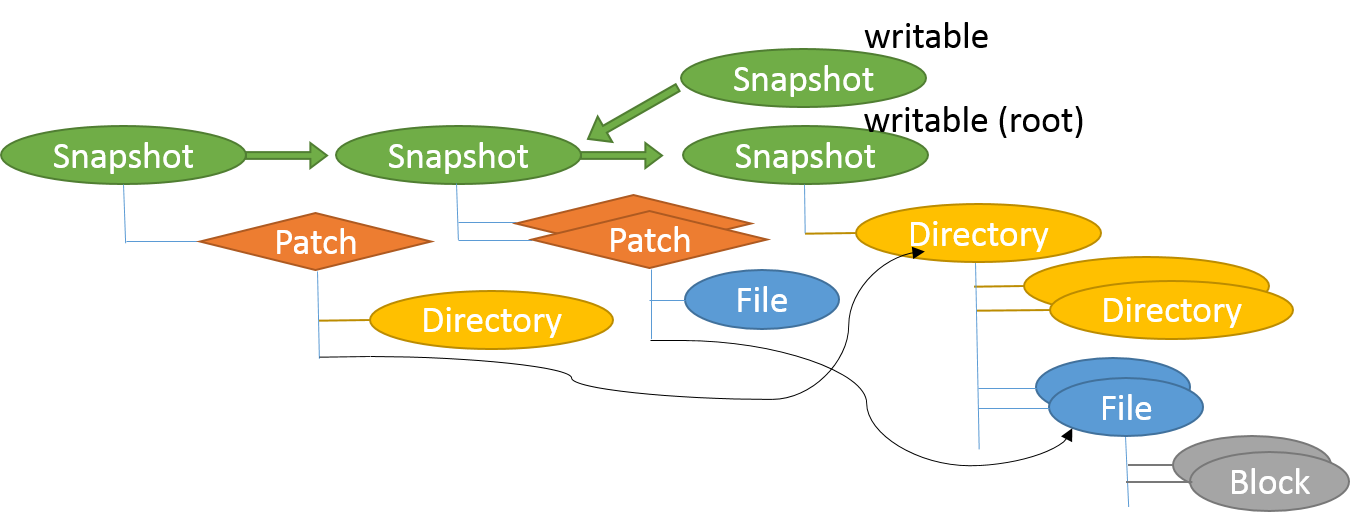
\includegraphics[width=0.9\textwidth]{Chapter-3/figs/fig2.png}
\caption{Basic Entities and Relations}
\label{fig:basic_entities}
\end{figure}

    \fref{fig:basic_entities} shows a basic view of the Kabi File System. The Kabi File System consists of 5 basic type of elements called node: the snapshot node, the patch node, the directory node, the file node and the block node. Nodes are referring to each other and forms a directed acyclic graph. In this implementation, each type of node is stored as a document in a MongoDB collection except for the patch node which is stored as a member object of a snapshot node. 

\section{Nodes}
    Nodes the basic entities defined by the internal interface. They are the inter-media objects between file system logic module and the storage abstraction module. The storage abstraction module manages how these nodes are stored in the MongoDB.
Block nodes are the very basic element in this file system. The block node is a representation of fixed-size binary data. Within a particular instance of the file system, the length of the byte string is immutable, while one can set different value for different instance of the file system on file system initialization. Though the size of data represented by the node is fixed, the node does not have to store that much bytes because the file system will add \'\textbackslash0\' padding at the end when necessary. In addition to the data field, a block node has two other field: a 128 bit hash of the byte string and a 32 bit rolling hash of the byte string. The structure of a typical block node is shown in \ref{tab:block_fields}.

\begin{table}
\caption{Fields in Block Node Object}
\label{tab:block_fields}
\begin{center}
\begin{tabular}{ll}
\toprule
field & remark\\
\midrule
id & the 128 bit SHA hash of bloack data\\
data & the block data\\
\bottomrule
\end{tabular}
\end{center}
\end{table}

    A file nodes is a representation of a certain file in the file system. In the Kabi File System, the content of the file is made up of several sections of variable length and each section is represented through a “data section” bson object. A file node consists a list of data sections and some other meta fields. Connecting the content of data section in order forms the content of the file. Each data section is correspond to exactly one block node and the block node may contribute only part of its binary data to the data section instead of its entire binary data. If only part of block node data is used by the data section, two integers will be specified to locate the start index and end index. \fref{fig:file_and_section} shows a file node consists of 3 data sections where the first data section contributes all 4 byte of corresponding block node data, the second section gets 2 bytes from its corresponding block node and the last section receives the first 2 bytes from its corresponding block node.

\begin{figure}[hbtp]
\centering
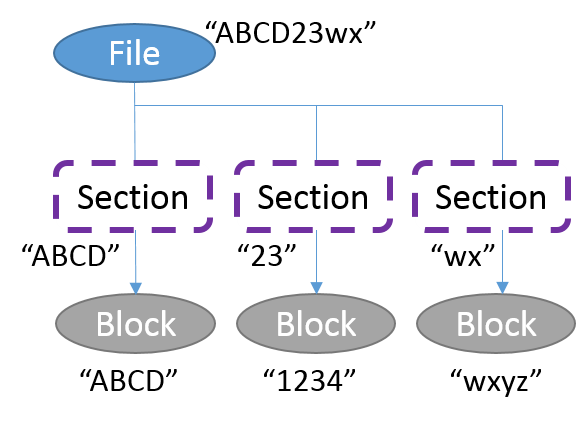
\includegraphics[width=0.5\textwidth]{Chapter-3/figs/fig7.png}
\caption{File Node, Section Object and Block Node}
\label{fig:file_and_section}
\end{figure}

	The detailed structure of a file node is shown in \ref{tab:file_fields}.

\begin{table}
\caption{Fields in File Node Object}
\label{tab:file_fields}
\begin{center}
\begin{tabular}{ll}
\toprule
field & remark\\
\midrule
mode & access mode of the directory\\
arc & a list of Section object\\
size & size of the file\\
owner & owner of the directory\\
gowner & group owner of the directory\\
modified & timestamp for last modification\\
\bottomrule
\end{tabular}
\end{center}
\end{table}

    The data section object is a Mongo bson object. It consists of three basic type as shown in \ref{tab:section_fields}, an object id referring to the associate block node, an integer value specifies the number of omitted leading bytes, another integer value specifies the index of last byte in block node. For the example shown in \fref{fig:section_and_block}, for the second block, the number of omitted leading bytes is 1, and the index of the last byte in block is 5.

\begin{figure}[hbtp]
\centering
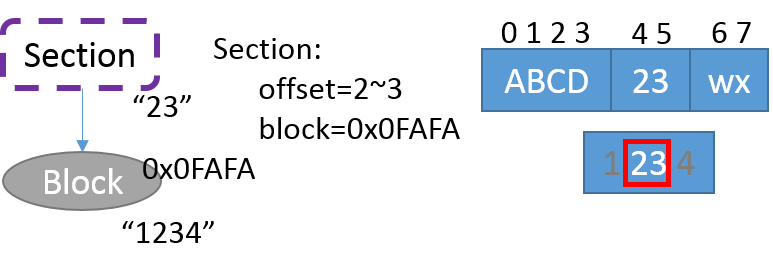
\includegraphics[width=0.9\textwidth]{Chapter-3/figs/fig9.png}
\caption{Section Object and Block Node}
\label{fig:section_and_block}
\end{figure}

\begin{table}
\caption{Fields in Section Object}
\label{tab:section_fields}
\begin{center}
\begin{tabular}{ll}
\toprule
field & remark\\
\midrule
id & id of corresponding \b{block}\\
roll & the 32 bit rolling hash of \b{block} data\\
omit & specify how many leading bytes in block will be omitted\\
offset & the offset of last byte in this \b{section}\\
\bottomrule
\end{tabular}
\end{center}
\end{table}

    Another important field of a file node is the “size”. It stores an integer value, representing the size of this file in bytes. When reading the file, \'\textbackslash0\' padding will be append to the end of files if the “size” value exceeds the total number of bytes in its data sections. On the contrary, if the total number of bytes in data sections exceeds the “size” vale, data will be truncated. This design allows faster creation and truncate operation to a file.

    A directory is represented by a directory node. The structure of a directory is similar to file node. It also consists of fields that store the meta information and a list of subnode object. Similar to the data section object in file node, subnode object is also stored as MongoDB BSON object. It may represent a sub directory or a subfile depending on the type of its referencing node. A subnode object contains a reference to a directory node or a file node, and a string field represents the display name of this subdirectory or subfile.

\begin{table}
\caption{Fields in Directory Node Object}
\label{tab:dir_fields}
\begin{center}
\begin{tabular}{ll}
\toprule
field & remark\\
\midrule
mode & access mode of the directory\\
arc & a list of SubNode object\\
owner & owner of the directory\\
gowner & group owner of the directory\\
modified & timestamp for last modification\\
\bottomrule
\end{tabular}
\end{center}
\end{table}

\begin{table}
\caption{Fields in SubNode Object}
\label{tab:subnode_fields}
\begin{center}
\begin{tabular}{ll}
\toprule
field & remark\\
\midrule
name & display name of the file or subdirectory\\
id & id of the file or subdirectory\\
\bottomrule
\end{tabular}
\end{center}
\end{table}


    The other two types of nodes are patch nodes and snapshot nodes, these two nodes are  related to the snapshot system and will be discussed in the related chapter.

\section{File System Operations}
    The file system logic module decomposes the FUSE file system calls to standard node operations defined by the internal interface. Most of the FUSE file system calls have been implemented in the Kabi File System, some of those important calls include getattr(), access(), read(), write(), rmdir(), unlink(), mkdir(), truncate(), flush(), open() and release(). Related node operations are addDirNode2db(), addFileNode2db(), addDataNode2db() and patch(). The former 3 methods write a node object into the database as a new node. The patch() method replaces an existing node with its new version.

\subsection{Read operations}
    getattr(), access() and read() are three important FUSE function. The access() function tests the existence and permission settings of a file or directory in the file system. getattr() returns the meta information about a file or directory. The read() function reads and return certain length of binary data at a specific offset.
The first step of a read operation is always finding the target file or directory node by path. In order to do so, the file system should parse the given path and find all corresponding nodes on the path in order from root directory to the target. The file system will start with the root directory, keep traversing subnode list and find the directory on the path until the algorithm hit the target or find it nowhere.

    This strategy is generally not satisfactory especially when the target hides deep in the directory tree. In such case, an access call will be mapped to a sequence of database queries on directory nodes and may become a bottleneck in performance. To solve this issue, a cache that stores the path-node relationship is introduced. With the help of the path-node cache, the file system will only query the database when the target directory or file cannot be found in the cache.

    The path-node cache is a move-to-front dictionary which maps the path string to directory node or file node. The cache has a fix capacity and assumes temporal locality in the access pattern. It uses move-to-front algorithm to keep frequently accessed hot item in the cache and remove those cold items that have not been accessed for long. The cache also assumes spatial locality: when accessing a file or directory, not only the file or directory itself is cached but all directories on the path, i.e. its parent and ancestor directories also go into the cache. Thus when visiting contents under the same directory later, the file system will find its parent node in cache.

    Once the file node is retrieved, reading the file is intuitive. The file system will traverse the data section list to find the id of block node associate with the read call and calculate the begin and end index of the bytes of the block content that will be copied to read buffer. After that the file system will query MongoDB for block nodes and copy requested data to buffer.

\subsection{Write operations}

\begin{figure}[hbtp]
\centering
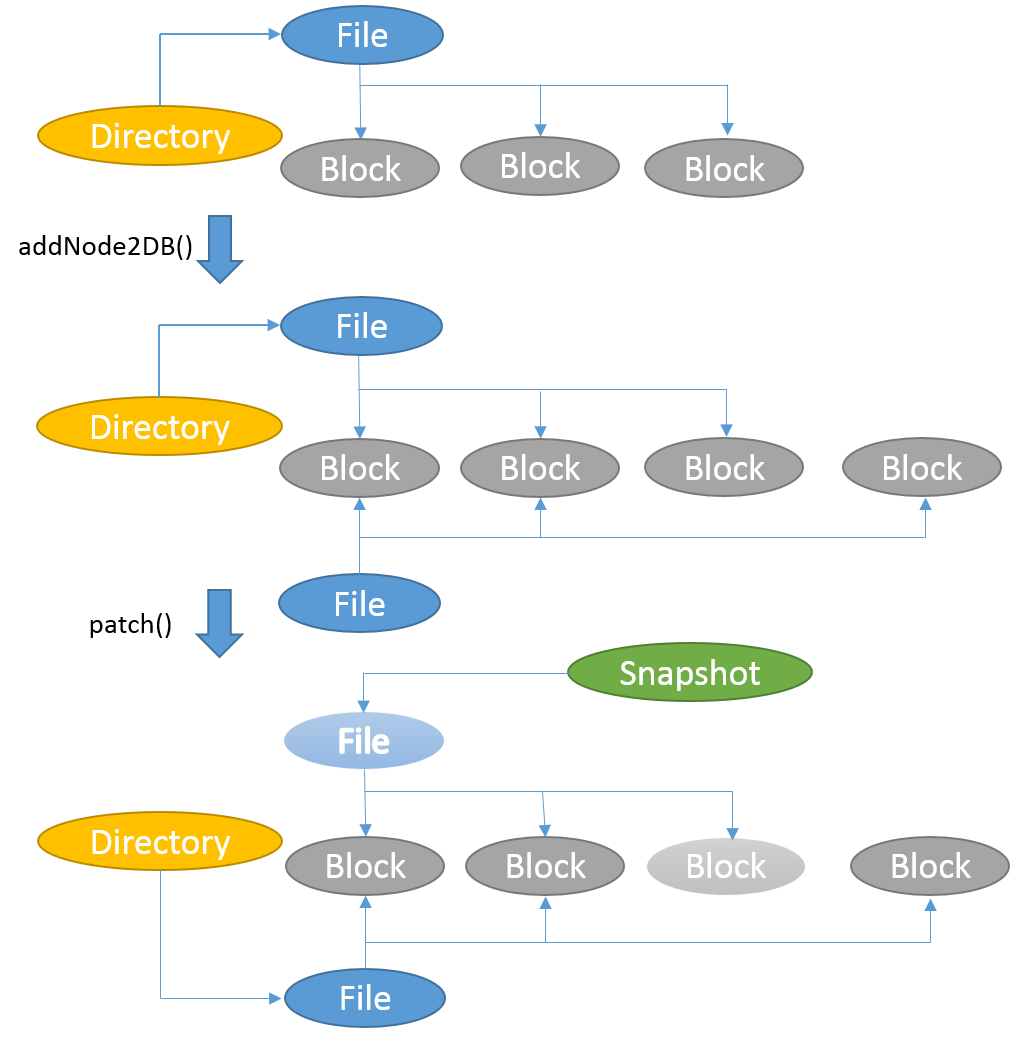
\includegraphics[width=0.8\textwidth]{Chapter-3/figs/fig10.png}
\caption{Copy-on-Write}
\label{fig:cow}
\end{figure}

    Write operations involves FUSE calls named write, chmod, chown, mkdir, unlink and rmdir. The write() call is the most important file system call that writes data into a file from some offset. Other functions change the meta information of a directory or file.

    Block nodes are designed to be immutable, file node and directory nodes uses copy-on-write strategy when an overwrite is requested. So when a overwrite to file node or directory node is requested, the file system will make a local copy of the node and apply the modification to this local copy. The file system will then upload that copy to remote and attach it to its parent directory replacing the pre-modified node as shown in the figure below. In this way, the old version of the node is saved for snapshot and read operation will not accidentally reads in a node in an incomplete state. As shownin \fref{fig:cow}, during this process, we use addNode2DB() operations to add a new node and use the patch() method to replace the old version with this new node.

	When writing a file, the write request will not flush data into persistent storage immediately but instead the data will be written into a local write buffer. Data in write buffer will be merged and subsequent write will overwrite previous buffered data when there is an overlap. When the file system receives a file close request or an explicitly flush request, data in buffer will be truncated into blocks and uploaded to remote servers. \fref{fig:buffer} shows how the buffer works.

\begin{figure}[hbtp]
\centering
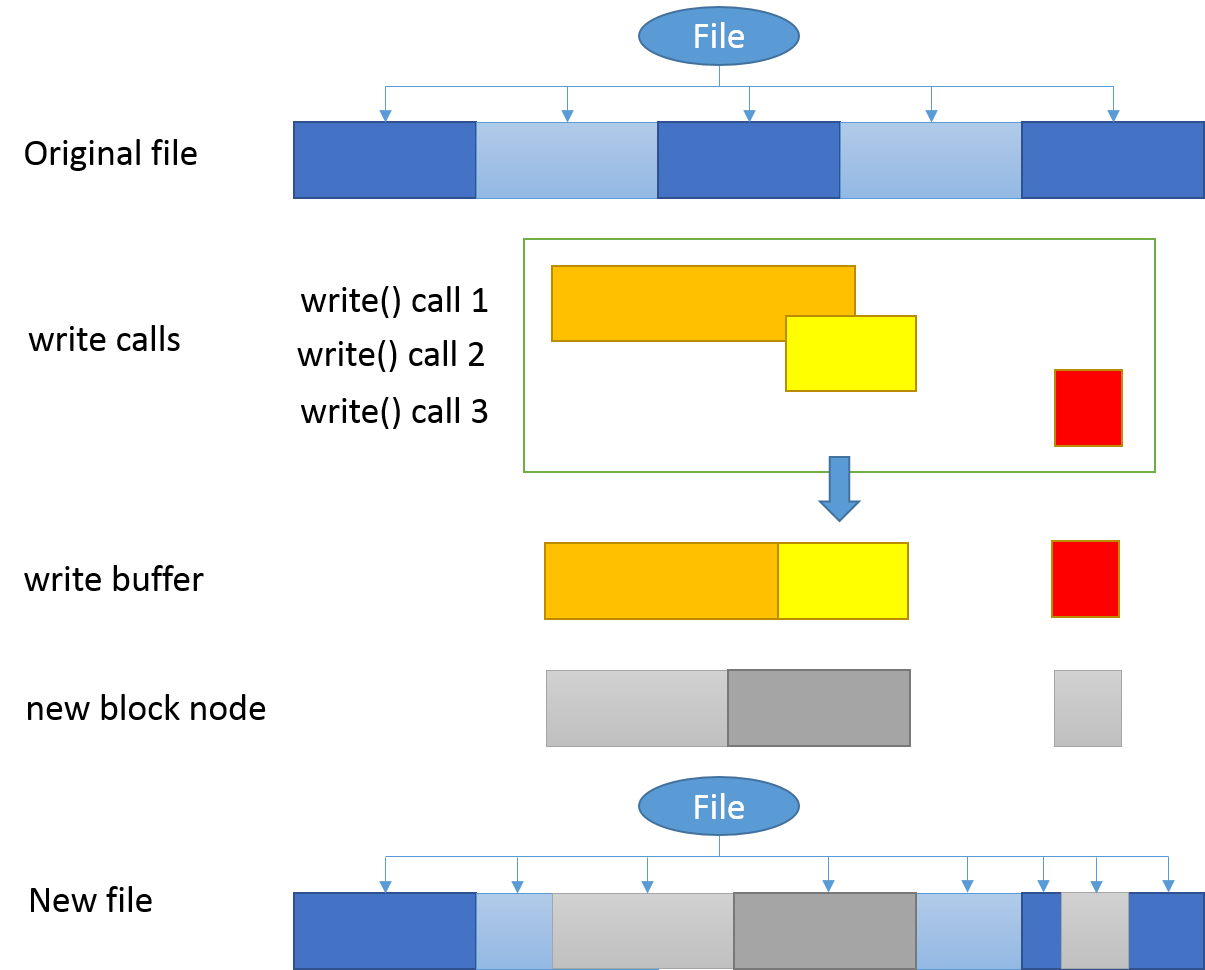
\includegraphics[width=0.8\textwidth]{Chapter-3/figs/fig11.png}
\caption{Write Buffer}
\label{fig:buffer}
\end{figure}

	During a flush, a data section may be unaffected, partly overwritten or entirely overwritten. Block node will be detached from the file if its representing data section has been entirely overwritten. The data section object will be truncated if this section is partly overwritten. The figure below shows the routine to write a file.


    Compared to the traditional copy-on-write snapshot file system which copies and overwrites the entire block whenever there is a byte change, this design can make use of the old block. Since the old block will be referenced by snapshots, reusing it in current view may save some storage for us.
However, there is a trade off between this saving and the overhead of such design. Each data section object requires 224 bit storage to store its SHA hash, rolling hash and begin/end indexes, each block node requires 128 bit to store its SHA id. But the overheads may be worthy. In extreme case, overwriting 2 bytes on the boundary of two block results in two new block to be created in traditional copy-on-write design while only one 2-byte block created in our design. With a block size of 2048 bytes and a file size of 20,480 bytes, this means 3798 bytes in saving.

\subsection{Deduplication}

    In a copy-on-write file system, there is rarely in-place modification to data. In most cases, making a change to the file system means creation of new nodes. On the other hand, creating a new block node is an expensive operation as it requires all data transferred to remote and a permanent reduction of the available space on the storage media.
We found that not all block node creation is necessary. Consider the following scenario, when some user program is trying to create a copy of some certain file to some other location. The program will reads in all data from file to buffer and then write the data in the buffer to another newly created file. As a result, the file system will experience a series of read() and write() function call, without acknowledging that these function calls are related. File system has no way to know that the block node it is going to write already exists in the file system and can be reused.

    By using SHA hash as the block node id, it is possible to find and eliminate blocks that contains duplicate data. Before a block of binary data is uploaded, the file system will query the database with its SHA, if a instance with same id is found, the file system will stop unloading the block node but directly return the id of existing node with same hash value.

    In this way, the file system not only can perform a copy operation efficiently but also find duplicated blocks or similar file and save space when saving them
\chapter{Snapshot}
\label{chap:snapshot}

    One of the major features in Kabi File System is the writable copy-on-write snapshot. A snapshot is a point-in-time copy of a defined collection of data.\cite{snapshot_def} A read only snapshot is an immutable copy of the file system data at a time spot, while a writable snapshot can be considered as a writable fork of such copy. Snapshot nodes are designed as the basic components of Kabi File System. The ``current'' view of the file system is also treated as a writable snapshot (the latest snapshot in default branch). This snapshot system focuses on reducing the storage space occupied by a snapshot.

    According to the Storage Networking Industry Association, three classic snapshot approachs include split-mirror, changed block, and concurrent.\cite{snapshot_types} The split-mirror approach copies every byte from source to snapshot. The process is time consuming hence it usually requires planning in advance. The changed block approach applies copy-on-write on the snapshot. The concurrent approach redirects IO request to different storage spaces associated with snapshots. Instead of making a copy and overwrite the copy, write IO request will be redirected a seperate storage space. While a read IO request will be redirected depends on whether the data has been changed since last snapshot.

    Our snapshot system uses a stratergy that is a mixture of copy-on-write and redirect IO. It uses enhanced copy-on-write stratergy on actual data and Redirect IO stratergy on meta data. In our snapshot system, most snapshots do not keep a copy of the entire file system but instead log the changes since the last snapshot. Such that the snapshot system can then recover the content of the a snapshot based on the previous snapshot and the log of changes, as shown in \fref{fig:snapshot_patch} The only exception is a special snapshot called head snapshot which contains contents of the entire file system at a particular time. Other snapshots are called referencing snapshot. They contain a reference to another snapshot and an array of patch objects. Each patch object in the array reflects a series of changes on a single file or a single directory since the last snapshot.

\begin{figure}[hbtp]
\centering
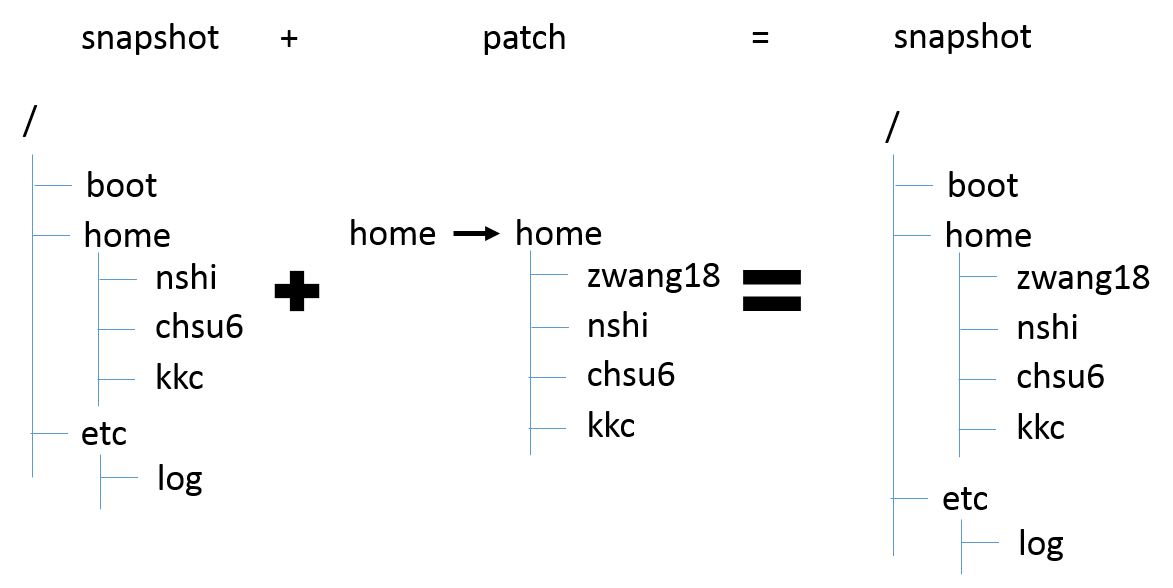
\includegraphics[width=0.8\textwidth]{Chapter-4/figs/fig23.png}
\caption{Snapshots and Patches}
\label{fig:snapshot_patch}
\end{figure}

\section{The Snapshot Tree}

	The snapshot system in Kabi File System uses a approach based on patches. Similar approach adpoted by ext3cow uses a reserved field in inode to reference the previous version inode shown in \fref{fig:snapfs_approach}. One advantage of the patch based approach is that it supports tree structured snapshots and writable snapshots.

\begin{figure}[hbtp]
\centering
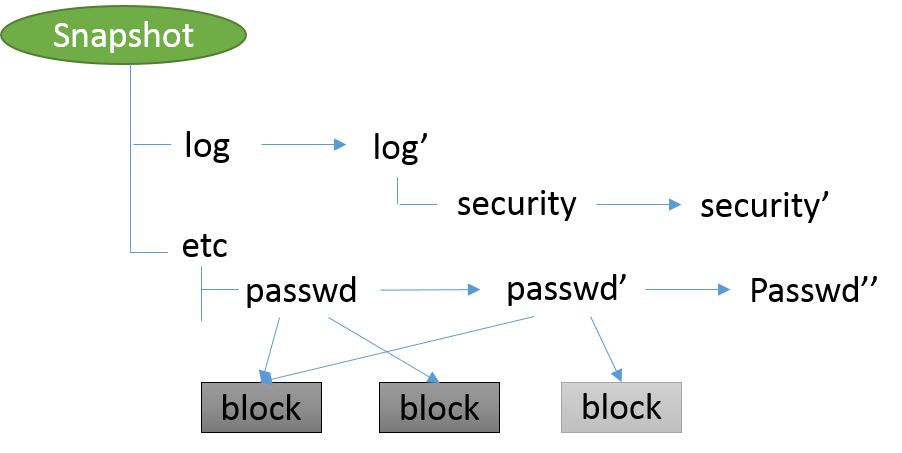
\includegraphics[width=0.7\textwidth]{Chapter-4/figs/fig24.png}
\caption{Snapshots in SnapFS}
\label{fig:snapfs_approach}
\end{figure}

    Snapshots in the Kabi File System are represented by snapshot node and forms an up-tree. In an up-tree, all child reference its parent. The following \fref{fig:snap_tree_example} shows an example of the snapshot tree. The left bottom node (node 0) is the root of the tree. The root of the snapshot tree is always the head snapshot.

\begin{figure}[hbtp]
\centering
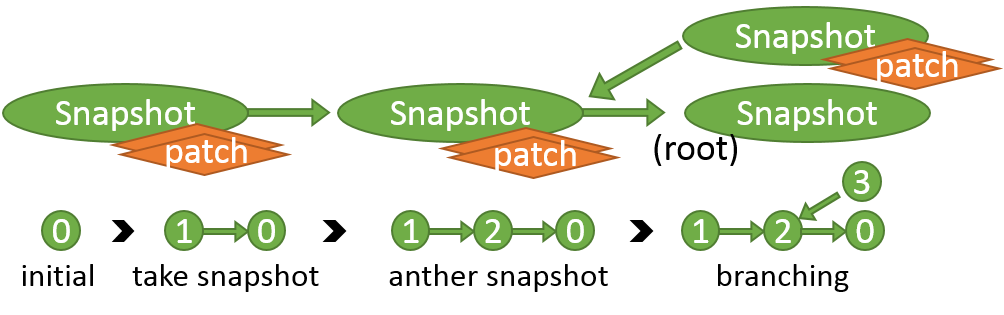
\includegraphics[width=0.8\textwidth]{Chapter-4/figs/fig13.png}
\caption{An example of snapshot tree}
\label{fig:snap_tree_example}
\end{figure}

    Initially, the file system contains a default writeable snapshot node (node 0 in \fref{fig:snap_tree_example}) representing the current view of the file system. This special snapshot called the head snapshot is the root of the snapshot tree and the only snapshot node that does not reference other snapshot. For initial state, any writes to the file system go directly into the head snapshot.
    
    After a snapshot is taken, a new snapshot node (node 1 in \fref{fig:snap_tree_example}) is created referring to the head snapshot node. Subsequent write operations will not only write data into the head snapshot but also submit patches to all snapshot connected to head snapshot, so as to reflect the difference between snapshot node 1 and its referencing node 0.

    Branching a snapshot is to create a writable copy of a existing snapshot. The branching operation is implemented by creating a new snapshot node referring the snapshot being forked. As shown in \fref{fig:snap_tree_example}, node 3 (the writable copy) is created and connected to snapshot node 2(the exisiting snapshot) in order to fork the file system based on snapshot 2.

    In the snapshot tree, each writable snapshot correspond to a branch. A branch consists of the writable snapshot (the current status of the branch) and its historical snapshots (the history of the branch). The main branch is the branch where the head snapshot node lies. \fref{fig:branches} shows the idea of branch. in the example, there are two branches in this 5-node snapshot tree. Node 0 is the root of the uptree so corresponds to the head snapshot. Thus node 1,2,0 forms the main branch. In the figure, nodes on the left corresponds to an older snapshot and nodes on the right corresponds to a more recent snapshot. Therefore in main branch, node 1 is the oldest snapshot while node 0 represents the latest state. Node 1 and 2 forms the history of main branch and node 0 is the current view of main branch. Node 4 is another writable snapshot and it belongs to a side branch. The side branch consists of node 1 (the oldest), node 2 (the second oldest), node 3 (the third oldest), and node 4 (most recent). Note that arrows between nodes reflect the referencing relations between snapshots, not the order of creation.

\begin{figure}[hbtp]
\centering
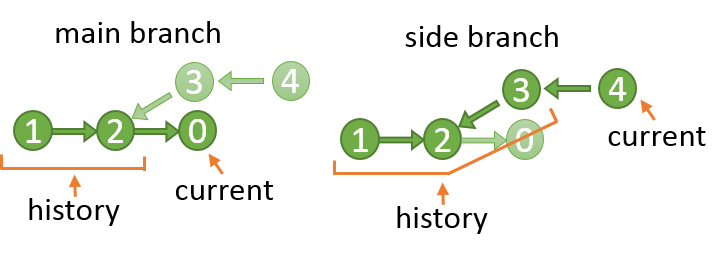
\includegraphics[width=0.65\textwidth]{Chapter-4/figs/fig22.png}
\caption{Branches}
\label{fig:branches}
\end{figure}

\section{Snapsho Nodes and Patch Object}

    As mentioned in previous section, there are two types of snapshot node in this file system, namely the head snapshot node and the referencing snapshot node.

    The head snapshot is special in the file system. It is the root of the up-tree and does not reference any other snapshots. Instead it stores the entire content of current view of main branch by referencing the directory node of the root directory. In this way, read access to the head snapshot node is straight forward and faster than any other snapshot. Because of this property, the head snapshot is recommended to represent the most frequently accessed snapshot or the current state of the default branch.

    On the other hand, a referencing snapshot does not reference its own root directory but it keeps a reference to another snapshot node and an array of patch objects. The array of patch objects represent the difference in content between this referencing snapshot and the referenced snapshot. Reading a referencing snapshot will first read the file system content in referenced snapshot and then lookup the patch list to find out if the content is changed in this snapshot. To write data, the referencing snapshot uploads the changed nodes into the database, build a patch object with both ids, upload and attach the patch to snapshot node in remote. This upload and attaching process is atomic and ensures the file system will not be left in a incomplete state. Once a referencing snapshot is referenced by some other snapshot nodes, it becomes read only snapshot. \fref{fig:root_and_nonroot} shows the structure of a head snapshot node (right) and the structure of a referencing snapshot (left).
    
\begin{figure}[hbtp]
\centering
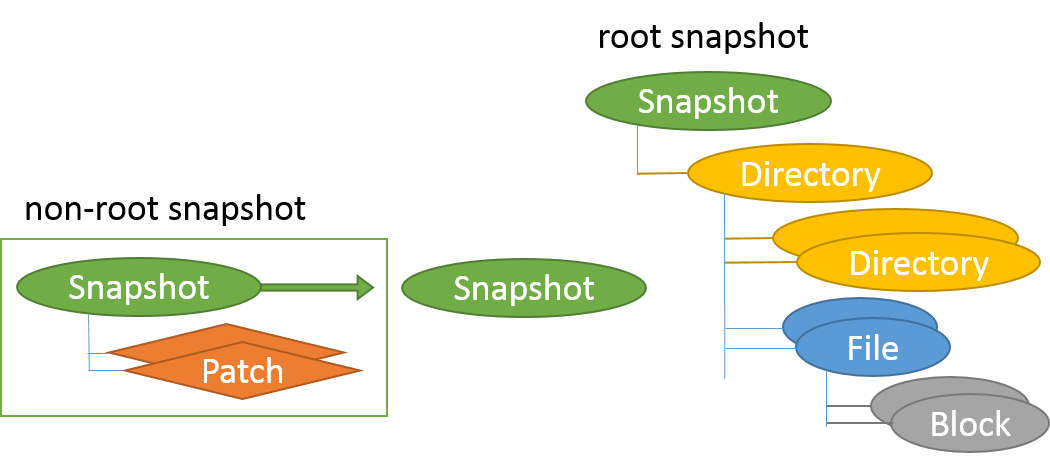
\includegraphics[width=0.75\textwidth]{Chapter-4/figs/fig12.png}
\caption{Root Snapshot and Non-root Snapshot}
\label{fig:root_and_nonroot}
\end{figure}

    A patch object reflects a single or a series of modification to a single node. The node can be either file node or one node. The patch object references a pair of file nodes or directory nodes. The two nodes referred are the target node (original version) and its replacement (changed version).

    \fref{fig:patches} demonstrates the way the patch systemworks. Snapshot 1 and 2 demonstrates how a directory changes between snapshots. The directory that is represented by node $d_2$ in snapshot 2 is now replaced by directory node $d_1$ in snapshot 1. In snapshot 2, the directory has a new subdirectory but the file under that directory remains unchanged. Hence the target node (node $d_2$) and replacement node (node $d_1$) have a reference to the same file node but the target node $d_2$ has one more reference to a directory node. In the example of snapshot ($a$) and snapshot ($b$), a file changes in both snapshot, its original version is $f_1$, the intermedia version in snapshot ($b$) is $f_2$ and final version is $f_3$ in snapshot ($a$). In snapshot $\alpha$ and snapshot $\beta$, file $f_3$ is replaced by $f_2$ in snapshot ($\beta$) and replaced by $f_1$ in snapshot ($\alpha$).  

\begin{figure}[hbtp]
\centering
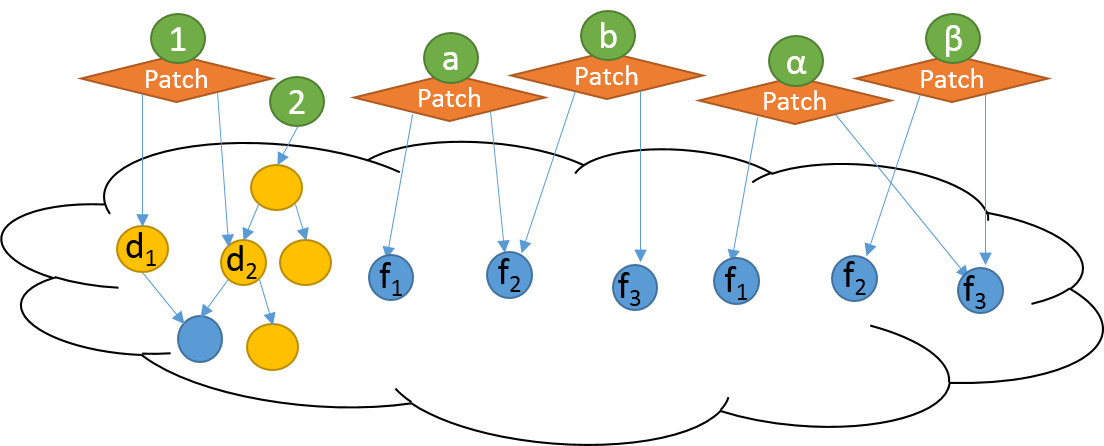
\includegraphics[width=0.75\textwidth]{Chapter-4/figs/fig14.png}
\caption{The Principle of Patches}
\label{fig:patches}
\end{figure}

\section{Snaphot related Operations}

    Operations in snapshot system involves read the content in a snapshot and make changes to (or write) a writeable snapshot. Make changes to the current view of the file system also involves snapshot write operation as the current view of the file system is also treated as a snapshot in Kabi file system.

\subsection{Read operations}

    When reading a file or a directory in the referencing snapshot, the file system must to do a large number of lookup in patch lists to ensure that the file system is referring to the correct version of the node. For instance, in \fref{fig:read_patches} , to read the file ``/a/d.txt'' in snapshot 1 shown in figure below, the file system will first read in ``/'' directory in head snapshot which is node 3. Then it transverses all involved snapshots (1 and 2) to see if there's a patch whose target node is node 3. Since no such patch is available, this means node 3 is the ``/'' directory node of all snapshot node (1, 2 and 3). Then the file system will look for “a” directory under node 3 and corresponding patches. In this example, there is a directory (node 9) with display name “a” under node 3 but there is also a patch to node 9 in snapshot 2. That means node 5 is the ``/a'' directory node of snapshot 0 while node 6 is the directory node for snapshot 1 and snapshot 2. Follow the same procedure, we will find node 8 is the ``/a/d.txt'' node in snapshot 2 but for snapshot 1 ``/a/d.txt'' represented by node 6.

\begin{figure}[hbtp]
\centering
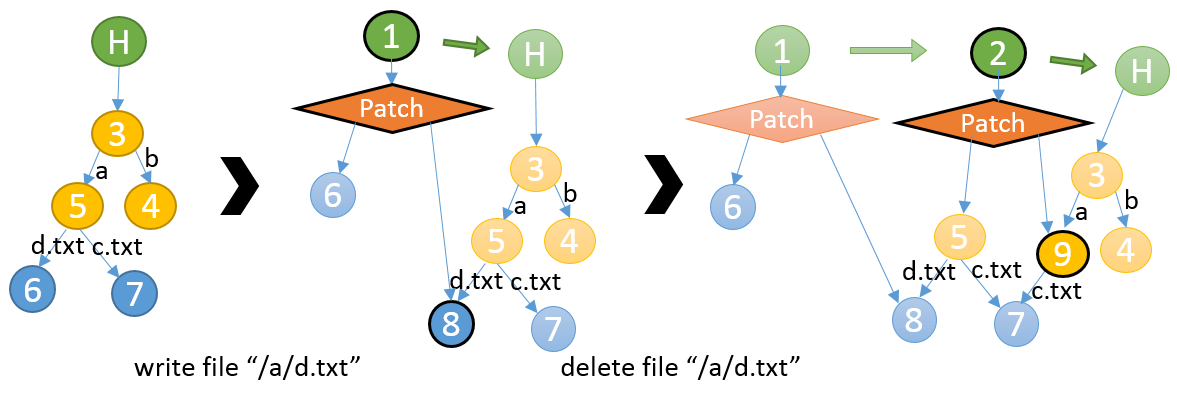
\includegraphics[width=0.5\textwidth]{Chapter-4/figs/fig18.png}
\caption{Read a snapshot}
\label{fig:read_patches}
\end{figure}

    As one can see, read operations rely on the patch lookup operation. To avoid query and traverse all involved snapshot and patch objects on every read operation, a local patch list is built and stored as hashtable in memory when a referencing snapshot node is mounted. The local patch list combines all patches that may be used for a node lookup. In the example shown in \fref{fig:combine_patch_list}, when mounting snapshot 3, a local patch list that contains all effective patches in snapshot 3 and 2 is created.

\begin{figure}[hbtp]
\centering
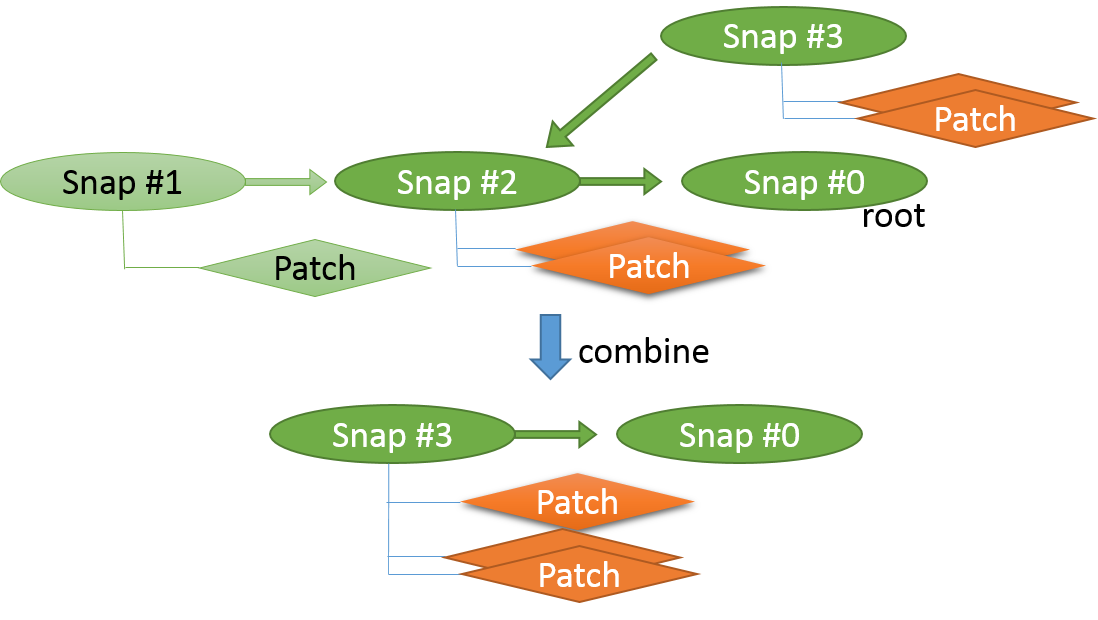
\includegraphics[width=0.8\textwidth]{Chapter-4/figs/fig15.png}
\caption{Combine Patch Lists}
\label{fig:combine_patch_list}
\end{figure}

    Not all patches in patch lists will be combined into a local patch list. Because patches are come from different patch lists, when they combine together some patches are mergeable and some are ineffective. For instance, in \fref{fig:merge} snapshot (a) and (b) the replacement node $f_2$ of a patch is also the target node of another patch, these two patch object can be merged into one local patch. Another example is snapshot ($\alpha$) and ($\beta$), the two patch shown in the figure have the same target node $f_3$. When snapshot ($\alpha$) is mounted, the patch in snapshot ($\beta$) will become ineffective and will not be read in.

\begin{figure}[hbtp]
\centering
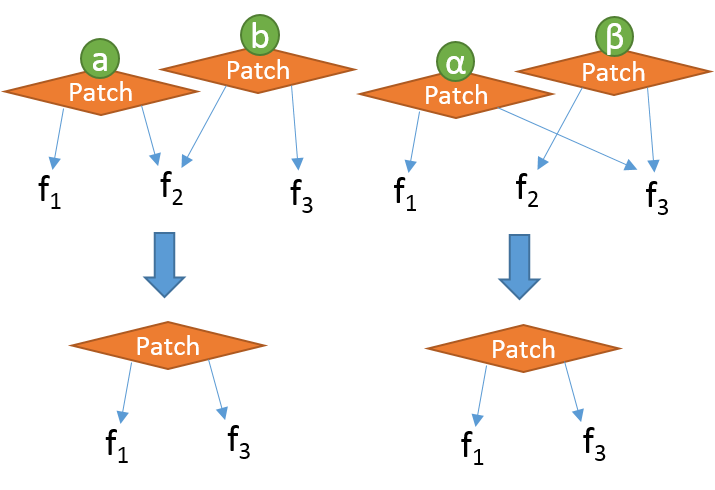
\includegraphics[width=0.7\textwidth]{Chapter-4/figs/fig19.png}
\caption{Merge Patches (Local)}
\label{fig:merge}
\end{figure}

\subsection{Write operations}

    In both copy-on-write snapshot system or redirect IO snapshot system, a file system entity (block, file, directory) may be referenced one or more times. Referencer could be snapshots or the ``current'' view of the file system. If an entity is referenced only once, write operation to that entity will be straight forward. This is a write operation within a snapshot. On the other hand, when an entity is referenced more than once, the snapshot system usually need special treatment to the write operation. Otherwise a direct in-place write will affect all referencer. In the snapshot system, we focus on the later case. If not otherwise specified, ``write operation'' in this section refers to those write calls whose target entities has been referenced more than once.

	\fref{fig:create_snapshots} briefly demonstrates how patch object and snapshots work with write operations. This example has 3 snapshots. Node 0 is the head snapshot node representing the current status of the main branch. Snapshot node 2 represents the initial status and node 1 is the intermediate status of main branch. Initially, the file system contains three directory ``/'', ``/a'', ``/b'' and two files ``/a/c.txt'', ``/a/d.txt''. In between the initial snapshot and the next snapshot, file ``/a/d.txt'' was overwritten so its representing node is changed by a patch. After snapshot 2 is taken, the file ``/a/d.txt'' was deleted. A new patch is attached to snapshot 2 to reflect this change.

\begin{figure}[hbtp]
\centering
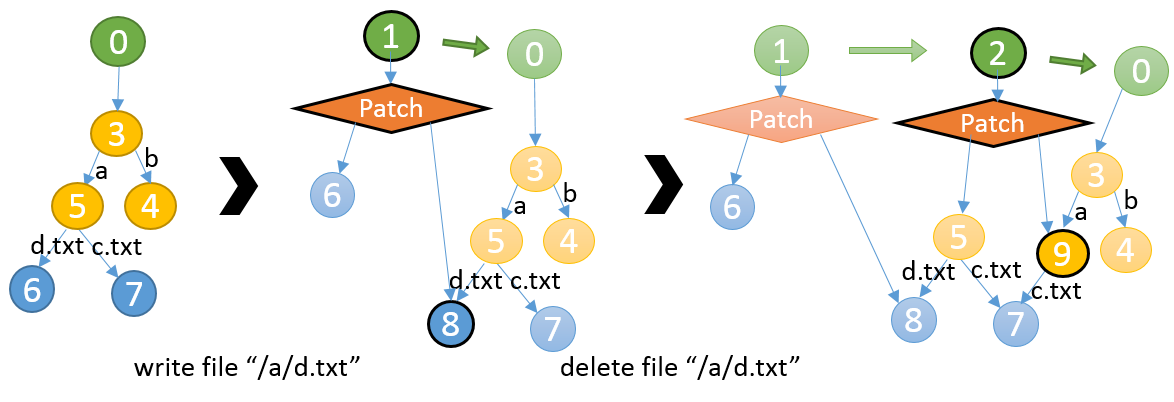
\includegraphics[width=0.95\textwidth]{Chapter-4/figs/fig26.png}
\caption{Example: Create Snapshots}
\label{fig:create_snapshots}
\end{figure}

    \fref{fig:take_snapshot_root} and \fref{fig:take_snapshot_nonroot} shows how to take snapshots on the main branch and side branchs.

    In order to take a new snapshot on the main branch, the file system will create a new snapshot node in between the head snapshot and its adjacent snapshot node. This newly created snapshots will have an empty patch list referencing the head snapshot. This new snapshot node will represent the status of this branch at the time it is created. The current state of the main branch is still the head snapshot.

\begin{figure}[hbtp]
\centering
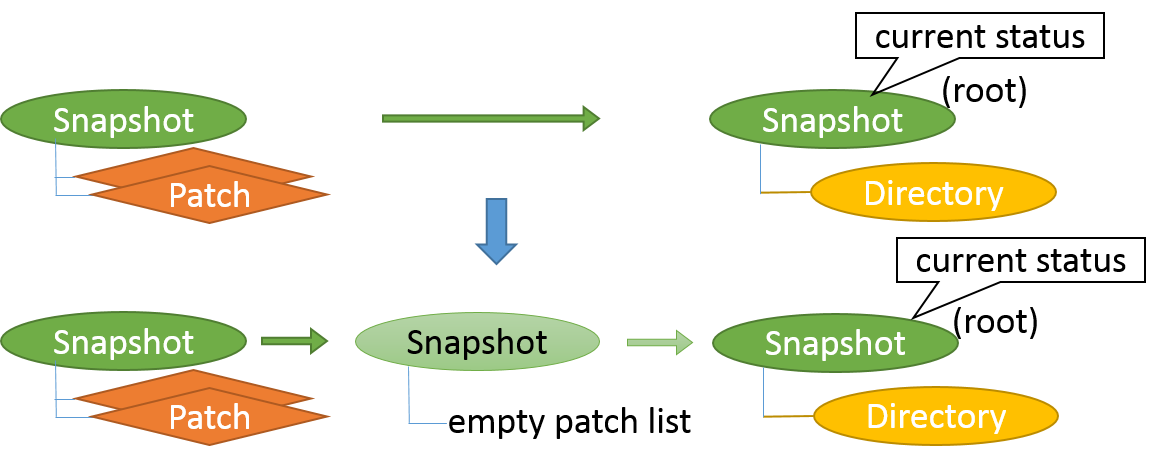
\includegraphics[width=0.8\textwidth]{Chapter-4/figs/fig20.png}
\caption{Take Snapshots on Main Branch}
\label{fig:take_snapshot_root}
\end{figure}
    
	To take a snapshot on a side branch, the file system will create a new snapshot node attached to the end of the side branch. The newly created snapshot node will reference the latest snapshot on this branch and have an empty patch list. After attaching to the branch, this snapshot will become the current status of this branch.

\begin{figure}[hbtp]
\centering
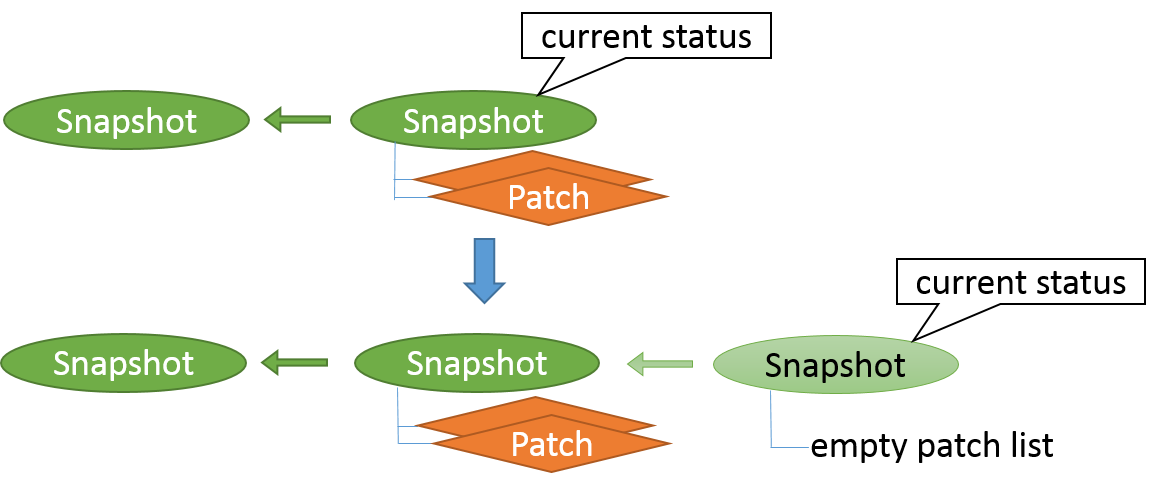
\includegraphics[width=0.8\textwidth]{Chapter-4/figs/fig21.png}
\caption{Take Snapshots on Side Branch}
\label{fig:take_snapshot_nonroot}
\end{figure}
    
    When writing a leaf referencing snapshot, the Kabi File System will submit new patches to that referencing snapshot to reflect the change. In the first example shown in \fref{fig:write_snapshot_node}, the file system is writing the head snapshot in main branch, replacing node X with its newer version Y. Node Y will replace node X directly in the head snapshot. In order to keep its previous version X in snapshot 2, a ``reverse'' patch object (Y-to-X) will be submitted to revert node Y back to its original version X. In this way, the head snapshot will have the new version Y while all other snapshots keep the old version X. In the second example, the file system is trying to replace node X with its new version Y in snapshot 3. Compared to the first example, the file system now can simply submit a X-to-Y patch to snapshot 3. In the third example, we demonstrate a walk around to writing an internal snapshot node by creating a branch based on that internal node and write to that branch.

\begin{figure}[hbtp]
\centering
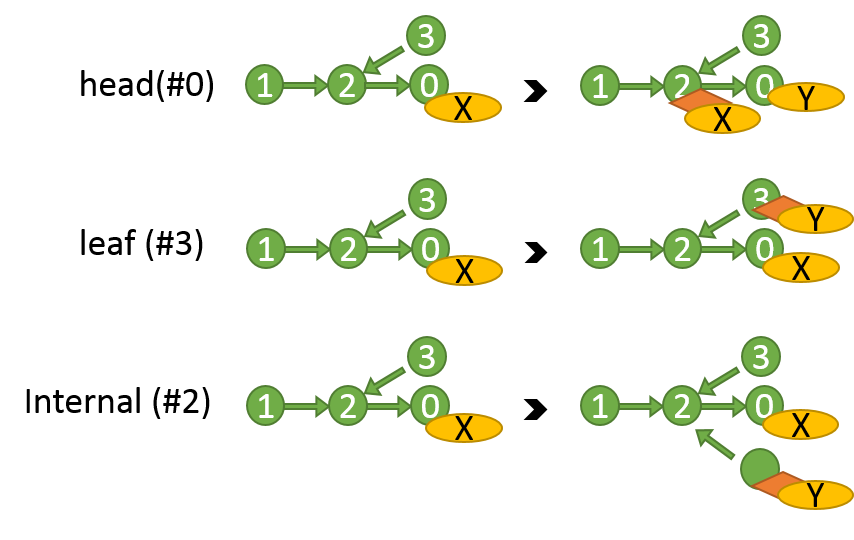
\includegraphics[width=0.7\textwidth]{Chapter-4/figs/fig17.png}
\caption{Write a Snapshot Node}
\label{fig:write_snapshot_node}
\end{figure}

    To create a branch based on the head snapshot, it is recommended to create a dummy snapshot first and then fork from that dummy node rather than branching the head snapshot directly. This is because a write operation to head snapshot will submit patches to all snapshot nodes connected to head snapshot node. Hence we wish to limit the number of snapshots connected to the head snapshot. If we fork the head snapshot directly then there will be multiple snapshot nodes connected on to the head snapshot node. \fref{fig:dummy_node} demonstrates this issue:

\begin{figure}[hbtp]
\centering
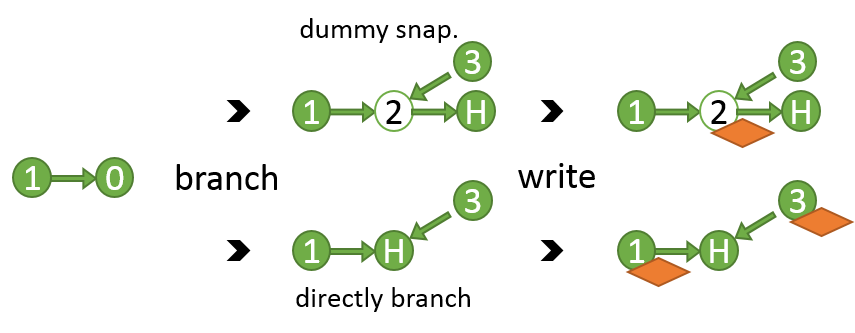
\includegraphics[width=0.8\textwidth]{Chapter-4/figs/fig16.png}
\caption{Branching Root Snapshot Node Directly}
\label{fig:dummy_node}
\end{figure}

	Generally, within a snapshot, each node (file or directory) should have no more than one patch associated with it. For example, a patch replacing node 0 with node 1 and a patch replacing node 1 with node 2 can be merged into one patch. This happens when a node is modified multiple times. For time and space efficiency, it is better to merge them into one patch.
	
\section{Enhancing Copy-on-Write and Deduplication}

	The copy-on-write strategy and file system deduplication improve space efficiency of the file system. File system deduplication finds and eliminates duplicated blocks and files while the classical copy-on-write strategy eliminates unnecessary copy of an unchanged block to snapshots.

\subsection{Motivation}

    A classical copy-on-write snapshot system applies copy-on-write at block level. As shown in \fref{fig:classic_cow}, unchanged blocks will not be copied to the snapshot.

\begin{figure}[hbtp]
\centering
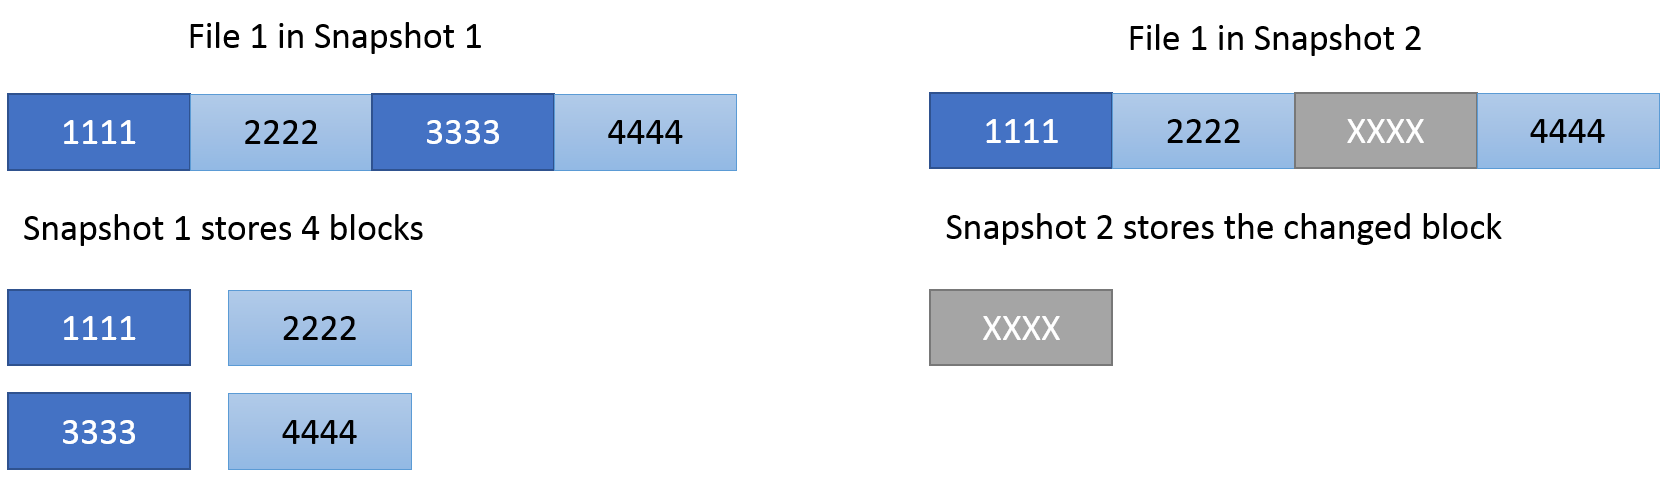
\includegraphics[width=0.8\textwidth]{Chapter-4/figs/fig4.png}
\caption{Classic Copy-on-Write}
\label{fig:classic_cow}
\end{figure}

    However, in reality it is not always an ideal solution. In many use cases like insertion or deletion, a write operation only affects a few bytes instead of a whole block. But a classic file system will rewrite all successor blocks in these scenarios. A classical snapshot system will make a copy of all successor blocks despite the fact that only very few bytes is changed. The following \fref{fig:issue_classic_cow} addresses this issue. In this example, a byte is inserted into the file at offset 8. In classical copy-on-write snapshot system, 2 successor blocks are treated as changed blocks and will be copied. However, actually, the data in those blocks did not change. They only moved one byte forward. In the figure we also demonstrates a potentially better approach.

\begin{figure}[hbtp]
\centering
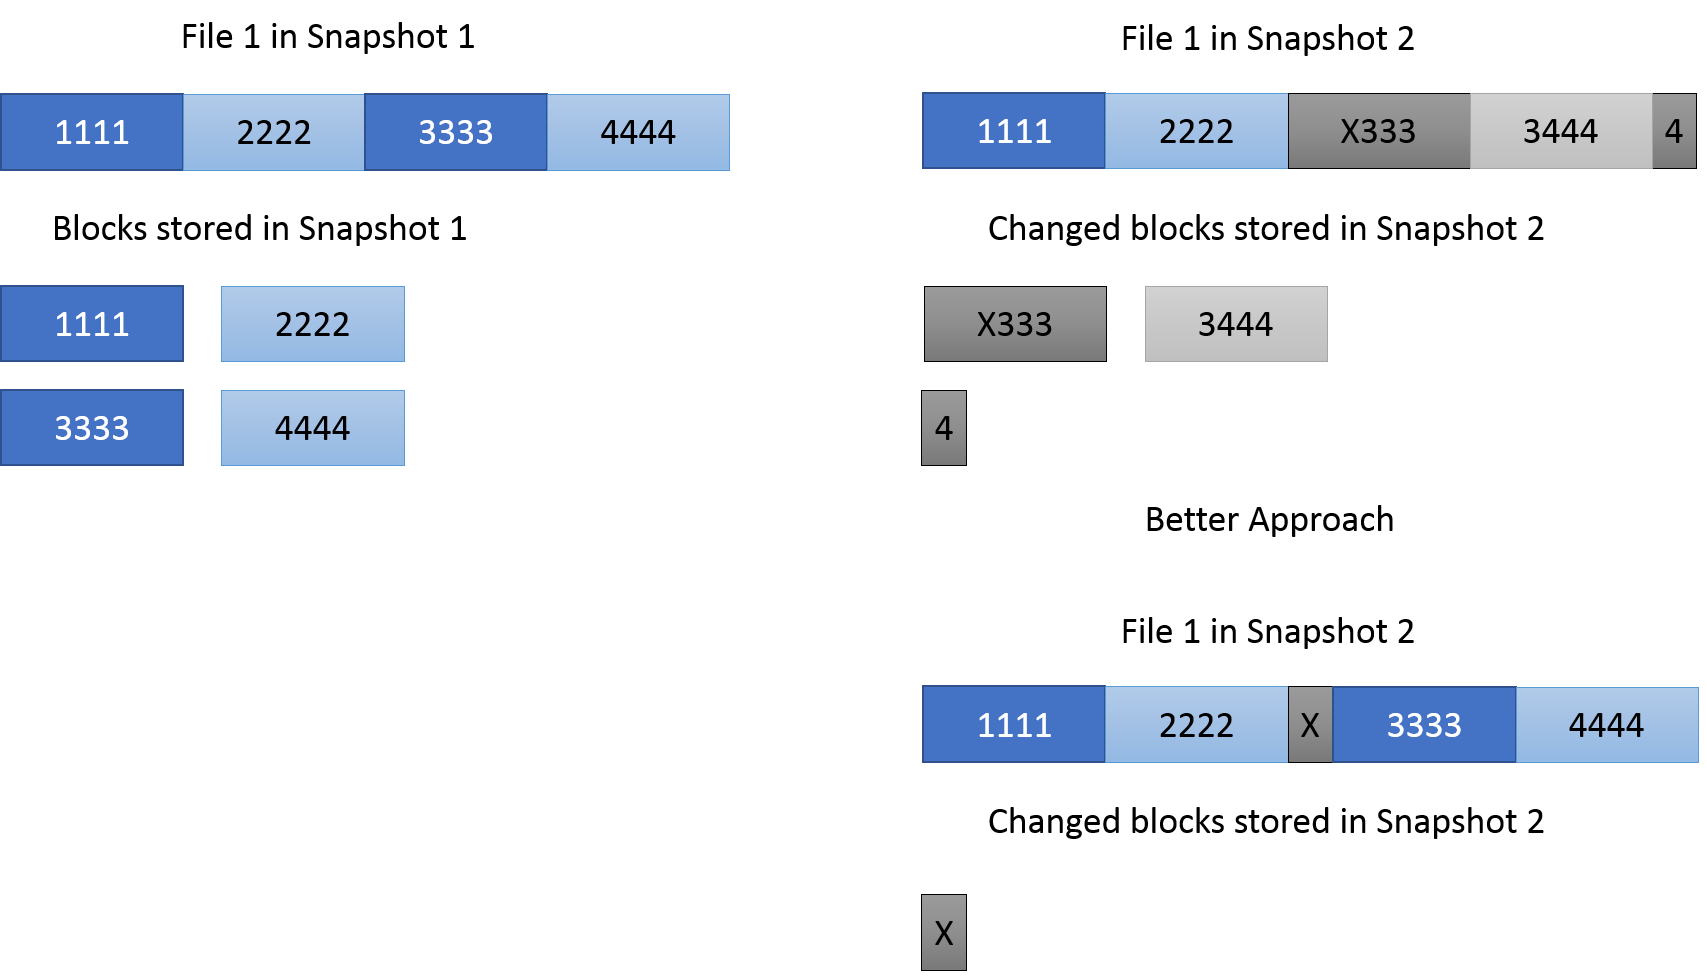
\includegraphics[width=0.8\textwidth]{Chapter-4/figs/fig5.png}
\caption{Issue in Classic Copy-on-Write}
\label{fig:issue_classic_cow}
\end{figure}
 
    To solve this problem, we have to let the file system be aware of the true intention of the end user. This is not straightforward because the POSIX standard uses only one file system call to handle all kinds of modification to a file. The only function of this file system call is to rewrite a part of a file.
    
    If the user program intend to insert a byte right in the middle of the file, the file system will receive a set of write calls to rewrite all later blocks in order to move original data 1 byte forward. The same behavior can also be observed when user program trying to rewrite the later half of the file. It is difficult for the file system to distinguish these two scenario. Access patterns can be used to guess the intention of an operation (i.e. an insertion usually results in a truncate call followed by a series of write() calls), but it is not an ideal solution as it depend on how the user program will behave. Therefore our major challenge is to identify the true intention of an write operation, whether should be an insertion or a complete rewrite.

    In this chapter we will show how to accomplish this goal by using the rsync algorithm.

\begin{figure}[hbtp]
\centering
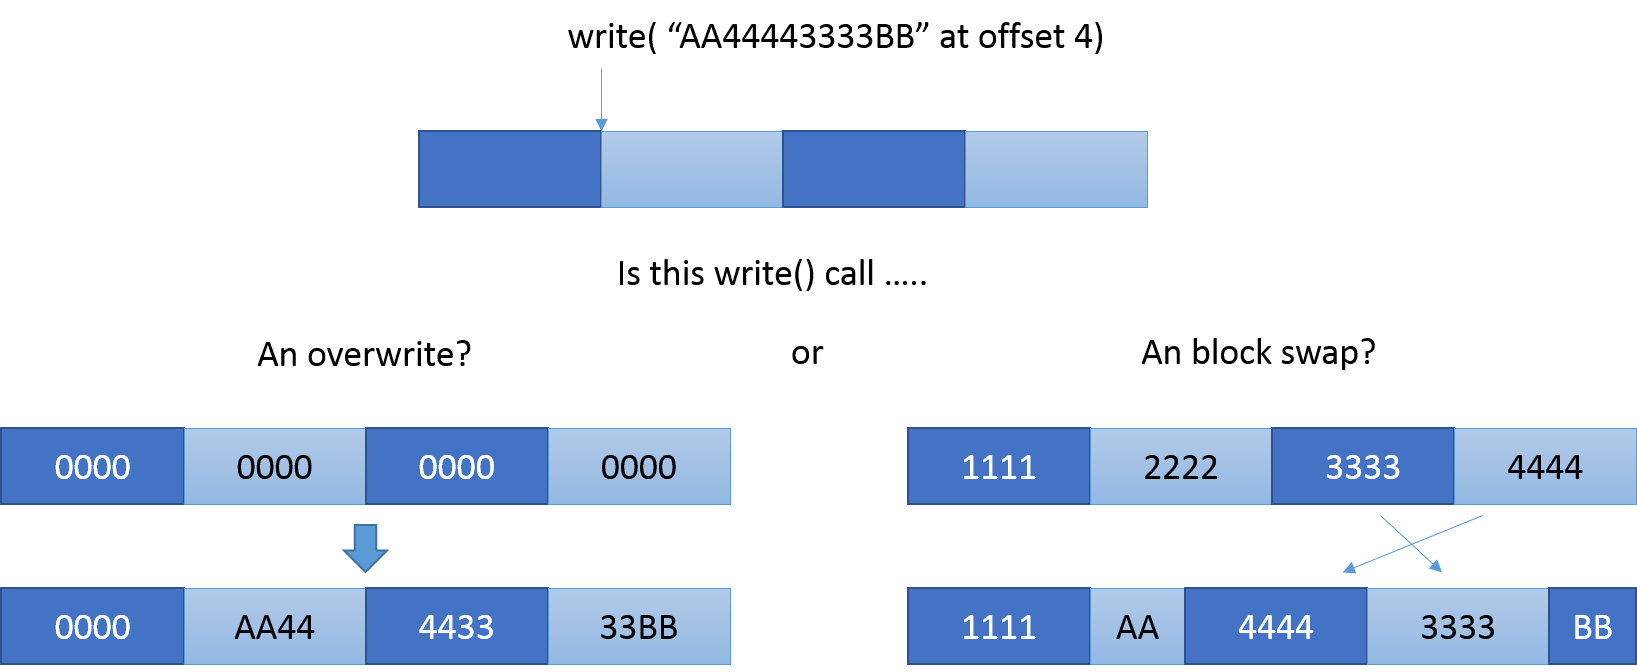
\includegraphics[width=0.8\textwidth]{Chapter-4/figs/fig6.png}
\caption{Identify the intention of write operations}
\label{fig:write_intention}
\end{figure}

\subsection{The rsync algorithm}

    As discussed in the previous section, in order to identify duplication in a better way, we need to have a mechanism to compare the data to be written into the file and the original data. 
    
    The rsync algorithm is originally designed for the efficient update of data over a high latency and low bandwidth link. Compared to brute force search and string search algorithms, rsync algorithm is much faster in practice and requires less data exchange between the remote server and local machine. These features make it suitable for a distributed file system. Because both time consuming file system and a high bandwidth consumption file system will become a bottleneck in the operating system.

    The basic flow of the rsync algorithm is to split the remote file into blocks of length $S$, calculate their rolling checksum and then send their them to the local machine. The local machine will search through local file to find all blocks of length $S$ bytes (at any offset, not just multiples of $S$) that matches the received rolling checksum. This can be done in a single pass very quickly since the rolling checksum only requires $O(1)$ time to compute checksum at offset k given the checksum at offset $k-1$.

\subsection{Enhancing the space efficiency}

    The Kabi File System uses the rsync algorithm to enhance the space efficiency of snapshots. It assumes that in most cases two different versions of the same file will share part of their data.

    In the Kabi File System, a section object in a file node contains not only the reference to the corresponding block, but also contains the rolling checksum of the block data. Before flushing the write buffer, the local machine will calculate the rolling checksum of data block at all possible offsets. The file system will compare these rolling checksums with those fetched from remote. If a match is found, the file system will then double check their SHA-1 hash to confirm that it is indeed a duplication.
    
    Once all data blocks have been examined, the local machine will send the ID of duplicated blocks and all remaining data back to the remote server.


\begin{figure}[hbtp]
\centering
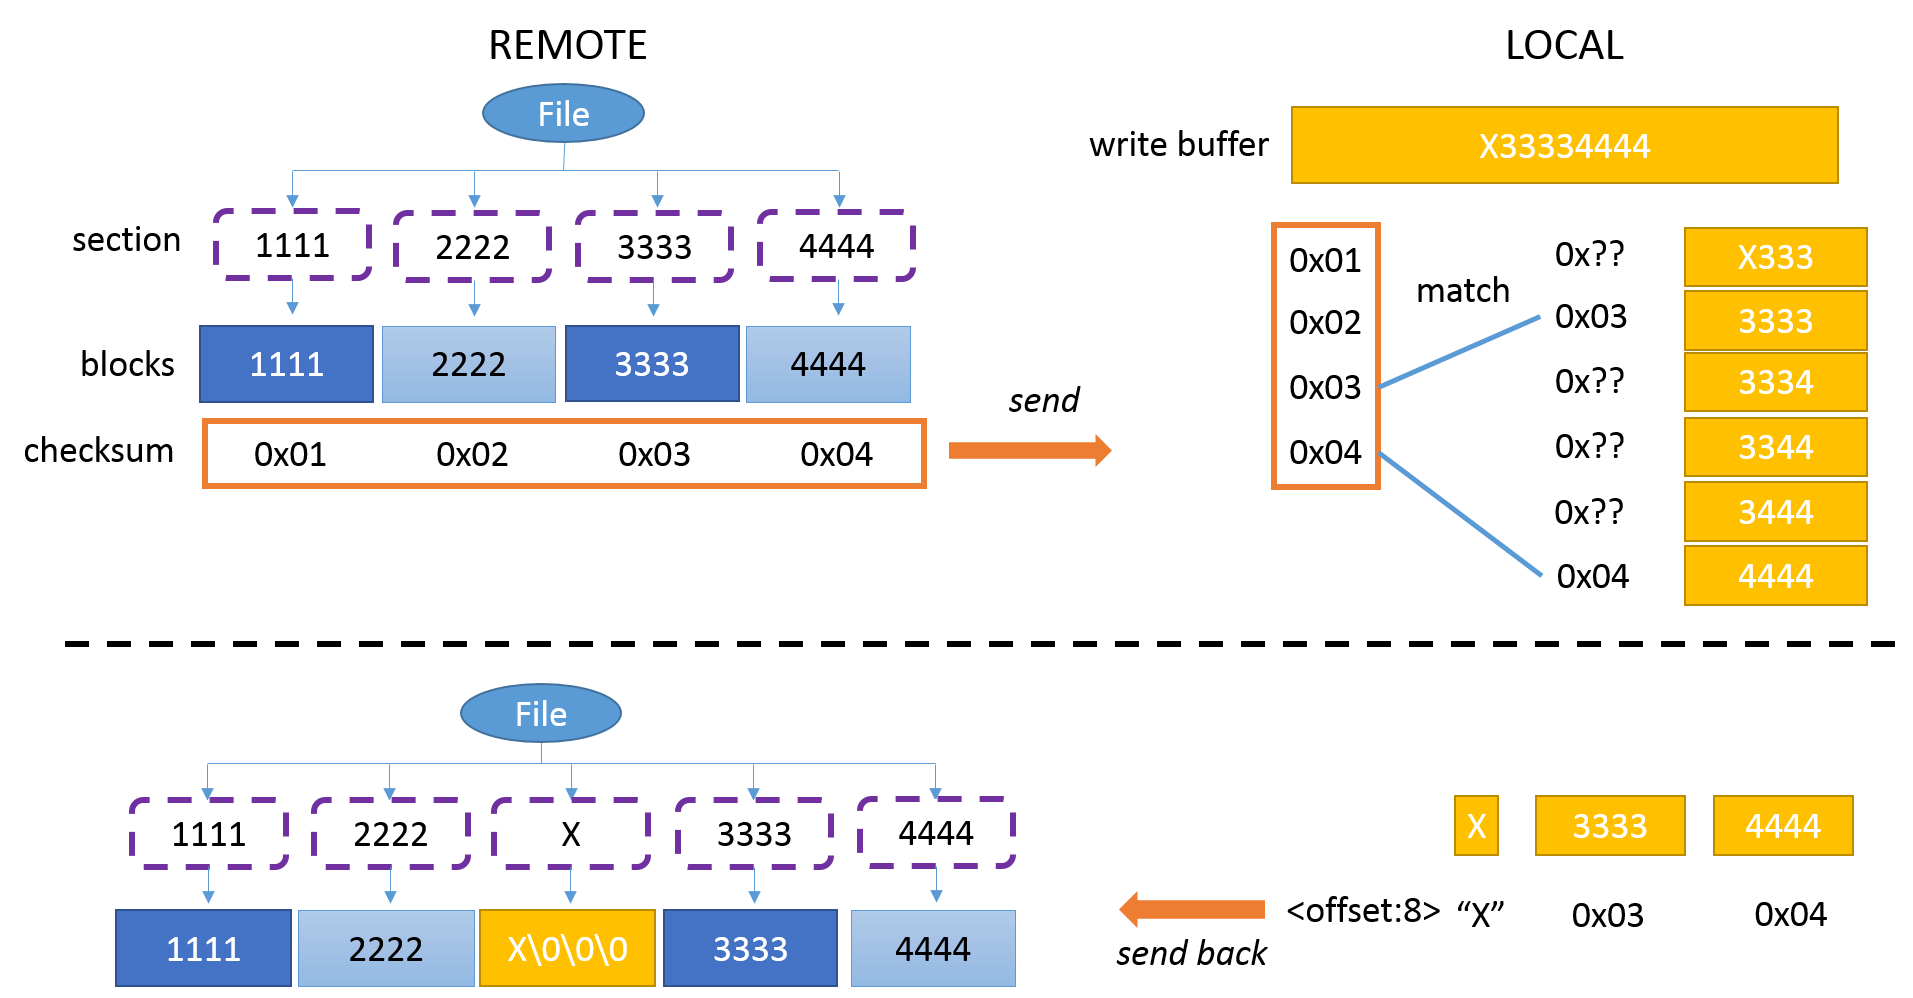
\includegraphics[width=0.9\textwidth]{Chapter-4/figs/fig25.png}
\caption{Using rsync to find unchanged blocks}
\label{fig:rsync}
\end{figure}

    During this process, the computational overhead is only the calculation and matching of rolling checksums. An important property of rolling checksum algorithm is that successive values can be computed in $O(1)$ time, thus ensuring that all rolling checksums can be calculated in $O(n)$ time. In contrast the benefits are a significant decrease in network flow and remote storage when there is duplicate data in buffer.

\section{Conclusion}

   In this chapter, we present the basic idea of this snapshot system and discuess some implementation details of the snapshot subsystem in Kabi File System. We demonstrated our efforts to make the snapshot system efficient in space usage. We also introduced the rsync algorithm to improve the snapshot system and the network performance.

\chapter{Snapshot Performence}
\label{chap:perform}

    The space occupied by a snapshot is an important measurement of how efficient the snapshot system is. In this chapter, we will focus on the actual space occupied by the snapshot using Kabi file system.
    
    A section that is not referring to a whole block like the third section in \fref{fig:rsync} will be named ``tuncated section'' here after.

    To monitor the space occupied by a snapshot, we will do experiments with the following steps:

\begin{enumerate}
	\item Initialize the file system with block size $B$.

	\item Generate a file with size $F$.

	\item Fill the file with sections and let a certain proportion ($P$) of the sections be truncated.

	\item Take a snaphot of the file.
	
	\item Insertion or overwrite random number of byte to the file at random offset. The offset parameter will be uniformly distributed between $0$ and $F$. The number of bytes being overwritten will be uniformly distributed from $1$ to largest possible value (i.e., until the end of the file).

	\item Take another snapshot and calculate the total space occupied by the second snapshot.

	\item Repeat above steps for 10,000 times to collect data (average value).
\end{enumerate}

    \tref{tab:sample_result} shows two sample result of such experiment. The first three columns in the table are the parameters of the experiment. The later four columns are the data gathered from the experiment. For example, the column labeled ``overwrite, classic'' means correspnding write operation is an overwrite and the algrithm used by snapshot system is classic Copy-on-Write.

    The first row in \tref{tab:sample_result} represents a experiment on a Kabi file system with 128 byte block size. The target file is a 12,608-byte file with 3\% sections truncated. The result shows that on average it takes a classic Copy-on-write snapshot system 3,288 bytes to take a snapshot after an overwrite operation. It takes 103 bytes more for a Kabi File System to take a snapshot under the same condition. When it comes to insertion, on average it only takes the Kabi File System 3,256 bytes to take a snapshot after an insertion while it costs almost 2 times more space for a classic copy-on-write snapshot system to do so.

    The result is intuitive. Because there's not much duplicated data in the overwrite scenario, storing the SHA hash, rolling checksum are overheads that makes the performance of Kabi File System a little lower than the classic approach. But in the insertion scenrio, lots of duplicated data can be found. The rsync algorithm is able to find the duplications but the classic approach is not able to do anything to that. So the Kabi File System gets a better perfromance this time.
    
    The second row in \tref{tab:sample_result} represents another experiment with file size equal to 126,080 bytes. It is obvious that when the file size becomes larger, the number space used to take a snapshot also become larger. But this makes comparasion between two experiments of different file size not so obvious. We introduce the normalized table, \tref{tab:norm}. The major difference between \tref{tab:norm} and \tref{tab:sample_result} is that in \tref{tab:norm} we use the size of the file to normailze the result data so that we can compare results from different experiments easier.

\begin{lscape} 
\begin{table}
\caption{Sample result of the experiment}
\label{tab:sample_result}
\begin{center}
\begin{tabular}{|c|c|c|c|c|c|c|}
\hline
\multicolumn{3}{|c|}{experiment parameters} & \multicolumn{4}{c|}{write operation and algorithm used} \\
\hline
block size & file size & truncated section & overwrite, classic & overwrite, Kabi & insert, classic & insert, Kabi\\
\hline
128 & 12608 & 3\% & 3288 & 3391 & 9530 & 3256 \\
\hline
128 & 126080 & 3\% & 31722 & 32205 & 94867 & 32557 \\
\hline
\end{tabular}
\end{center}
\end{table}

\begin{table}
\caption{Normalized data}
\label{tab:norm}
\begin{center}
\begin{tabular}{|c|c|c|c|c|c|c|}
\hline
\multicolumn{3}{|c|}{experiment parameters} & \multicolumn{4}{c|}{write operation and algorithm used} \\
\hline
block size & file size & truncated section & overwrite, classic & overwrite, Kabi & insert, classic & insert, Kabi\\
\hline
128 & 12608 & 3\% & 0.2607 & 0.2689 & 0.7558 & 0.2582 \\
\hline
128 & 126080 & 3\% & 0.2516 & 0.2554 & 0.7524 & 0.2582 \\
\hline
\end{tabular}
\end{center}
\end{table}
\end{lscape}

\subsection{Block Size and File Size}
\begin{lscape} 
\begin{table}
\caption{Sample result of the experiment}
\label{tab:sample_result}
\begin{center}
\begin{tabular}{|c|c|c|c|c|c|c|}
\hline
\multicolumn{3}{|c|}{experiment parameters} & \multicolumn{4}{c|}{write operation and algorithm used} \\
\hline
block size & file size & truncated section & overwrite, classic & overwrite, Kabi & insert, classic & insert, Kabi\\
\hline
128 & 704 & 17\% & 0.4531 & 0.5127 & 0.8338 & 0.2983 \\
\hline
128 & 1408 & 17\% & 0.3514 & 0.3934 & 0.7933 & 0.2962 \\
\hline
128 & 2112 & 17\% & 0.3129 & 0.3532 & 0.7789 & 0.2964 \\
\hline
128 & 3520 & 17\% & 0.2884 & 0.3213 & 0.7702 & 0.2972 \\
\hline
128 & 7040 & 17\% & 0.2681 & 0.2949 & 0.7589 & 0.2955 \\
\hline
128 & 14008 & 17\% & 0.2593 & 0.2828 & 0.7545 & 0.2957 \\
\hline
\end{tabular}
\end{center}
\end{table}
\end{lscape}
\subsection{Truncate Ratio}
\begin{lscape} 
\begin{table}
\caption{Sample result of the experiment}
\label{tab:sample_result}
\begin{center}
\begin{tabular}{|c|c|c|c|c|c|c|}
\hline
\multicolumn{3}{|c|}{experiment parameters} & \multicolumn{4}{c|}{write operation and algorithm used} \\
\hline
block size & file size & truncated section & overwrite, classic & overwrite, Kabi & insert, classic & insert, Kabi\\
\hline
128 & 12800 & 0\% & 0.2596 & 0.2645 & 0.7547 & 0.2495 \\
\hline
128 & 12800 & 10\% & 0.2600 & 0.2752 & 0.7558 & 0.2750 \\
\hline
128 & 12800 & 18\% & 0.2599 & 0.2856 & 0.7557 & 0.3002 \\
\hline
128 & 12800 & 33\% & 0.2606 & 0.3071 & 0.7569 & 0.3513 \\
\hline
128 & 12800 & 46\% & 0.2616 & 0.3290 & 0.7579 & 0.4026 \\
\hline
128 & 12800 & 57\% & 0.2616 & 0.3500 & 0.7583 & 0.4532 \\
\hline
128 & 12800 & 71\% & 0.2596 & 0.3792 & 0.7530 & 0.5252 \\
\hline
128 & 12800 & 82\% & 0.2579 & 0.4089 & 0.7505 & 0.5980 \\
\hline
128 & 12800 & 91\% & 0.2593 & 0.4417 & 0.7536 & 0.6758 \\
\hline
128 & 12800 & 100\% & 0.2601 & 0.4737 & 0.7561 & 0.7536 \\
\hline
\end{tabular}
\end{center}
\end{table}
\end{lscape}
\subsection{Conclusion}

\chapter{Conclusion}
\label{chap:conclusion}

    In this thesis, we presented the design of a new distributed file system with snapshot capability. We also built a proof of concept implementation of such design using MongoDB, FUSEi and other techniques. We designed and implemented a new copy-on-write snapshot system and try to improve its efficiency in many ways. We evaluated the snapshot system by testing variables that affects the efficiency of the snapshot and we also came up with some explaination of how these factors affect the efficiency.

    We believe the major contribution of this thesis are the design of the proposed file system, the design of the snapshot subsystem, and the evaluation of the snapshot subsystem.

\section{Future work}

     We already knew that the proportion of truncated section affects the efficiency significently. It is possible that a large block size will increase the proportion of truncated section in long run. Further more, We may also want to find out the optimal block size when given the distribution of file size stored on the Kabi File System.

     In the file system proposed, the proportion of truncated section will increase though out the time. It is possible to merge adjacent truncated sections to reduce the occuernce of truncated section so as to improve the performance. Futher more, it may be worthy to rebuild a file node filled with truncated sections at some point, such that the new file node contains the same data but less truncated section.

     (SWITCHABLE branches)
     (overhead of MongoDB nonlinear addressing)




%%---------------------------------------------------------------------------%%
%%  Bibliography 

%%  You can use the bibitem list.
%\bibliographystyle{unsrt}
%\begin{thebibliography}{99}
%\bibitem{cb02}
%Casella, G. and Berger, R.L. (2002)
%\newblock {\it Statistical Inference, Second Edition.}
%Duxbury Press, Belmont, CA.
%
%\bibitem{t06}
%Tsiatis, A.A. (2006)
%\newblock {\it Semiparametric Theory and Missing Data.}
%Springer, New York.
%
%\end{thebibliography}

%% or use BibTeX
\bibliography{thesis}{}
\bibliographystyle{plain}

%%---------------------------------------------------------------------------%%
% Appendices
%\appendix

%\chapter{Lorem Ipsum}

\section{A First Section}

\paragraph{Filler Text} \lipsum[1-6]
%
\begin{figure}
  \centering
  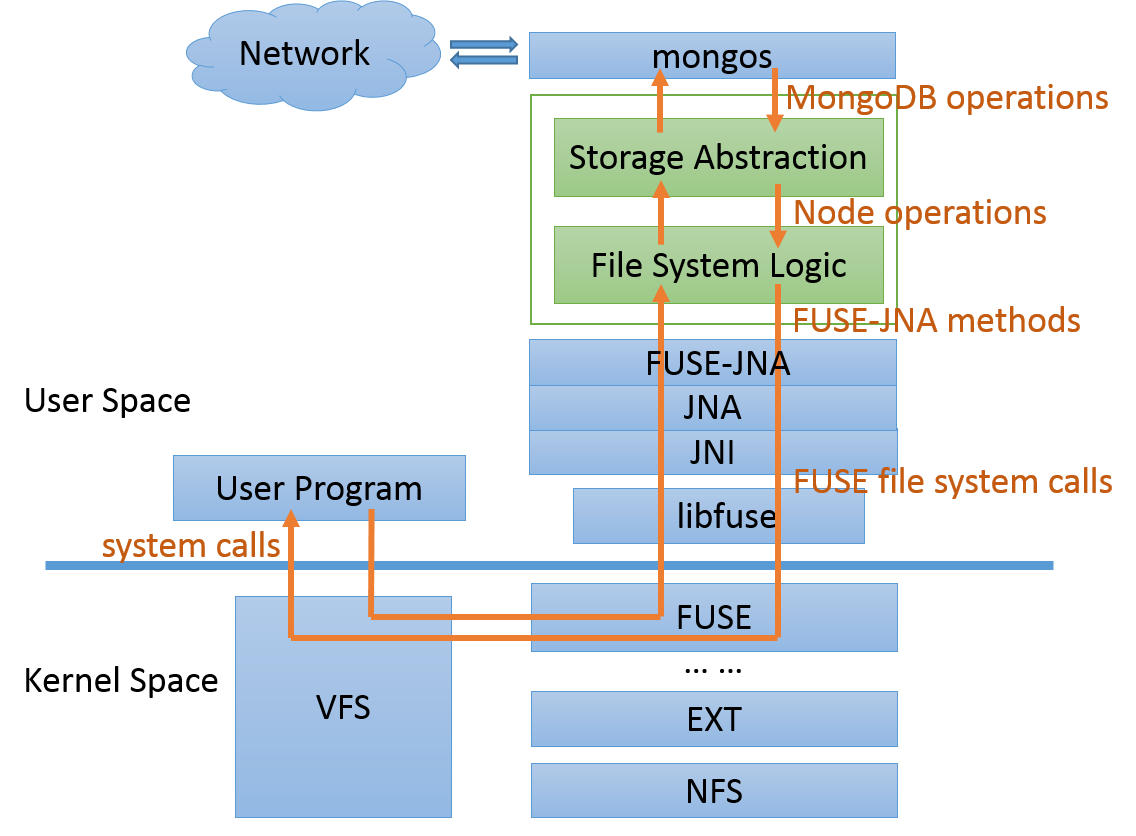
\includegraphics[width=0.6\textwidth]{Chapter-3/figs/fig1.png}
  \caption{A figure in the appendix.}
  \label{fig:app}
\end{figure}
%
\lipsum[7-10]
\begin{table}
  \caption{A table in the appendix.}
  \label{tab:app}
  \begin{center}
    \begin{tabular}{lc}
      \toprule
      System & Author \\
      \midrule
      \TeX   & Donald Knuth   \\
      \LaTeX & Leslie Lamport \\
      \bottomrule
    \end{tabular}
  \end{center}
\end{table}
%

\section{A Second Section}

\lipsum[14-15]




%%---------------------------------------------------------------------------%%
\backmatter


\end{document}
